%%%%%%%%%%%%%%% Updated by MR March 2007 %%%%%%%%%%%%%%%%
\documentclass[12pt,a4paper]{article}
\usepackage{a4wide}
\usepackage{graphicx}
\usepackage{amssymb}
\usepackage{amsmath}
\usepackage{amsfonts}
\usepackage[utf8]{inputenc}
\usepackage[left=2cm,right=2cm,top=2cm,bottom=2cm]{geometry}

\newcommand{\al}{$<$}
\newcommand{\ar}{$>$}

\parindent 0pt
\parskip 6pt


\author{Ben O'Neill}

\begin{document}

\thispagestyle{empty}
\rightline{\large \textbf{Benjamin O'Neill}}

\vfil

%cover page
\centerline{\Large\bf Efficient Asymmetric Cryptography for}
\centerline{\Large\bf RFID Access Control}
\vspace{0.4in}
\centerline{\Large Computer Science Tripos - Part II}
\vspace{0.3in}
\centerline{\Large Emmanuel College}
\vspace{0.3in}
\centerline{\Large 2018}
\vfil
\pagebreak

%Proforma
\thispagestyle{empty}
\centerline{\Large Proforma}

\noindent
\begin{minipage}{0.3\textwidth}
\raggedright
{\bf Name:}\\
{\bf College:}\\
{\bf Project Title:}\\
{\bf Examination:}\\
{\bf Word count:}\\
{\bf Project Originator:}\\
{\bf Project Supervisor:}
\end{minipage}
\begin{minipage}{0.7\textwidth}
%\raggedleft
Benjamin O'Neill\\
Emmanuel College\\
Efficient Asymmetric Cryptography for RFID Access Control\\
Computer Science Tripos Part II - 2018\\
TODO\\
Dr Markus Kuhn\\
Dr Markus Kuhn
\end{minipage}

\vspace{0.3in}
{\large\bf Original aims of the project}\\
As outlined in the project proposal (TODO: link to), the original aim of the project was to consider practical options for smartcard authentication systems based on asymmetric cryptography. 
 
The motivation for this to be able to propose a feasible replacement for the current university access control system based on Mifare classic, which has been shown to be insecure. An asymmetric implementation would also be convenient in a number of other ways, as outlined in (TODO: reference). After an approach and protocol is chosen, a working prototype implementation would be produced using programmable Java Cards.

\vspace{0.3in}
{\large\bf Work completed}\\
After briefly looking at a few protocols, and becoming accustomed to the development process, I produced a working implementation of the Opacity ZKM (Zero Key management) protocol, which required implementing the protocol both on the programmable smartcard and on the host, which was a typical desktop PC with a USB card reader. 

The implementation was then refined to improve the authentication speed and fix any tearing issues or security flaws.

\vspace{0.3in}
{\large\bf Special difficulties faced}\\
%NOTE: Not sure how much of this I should keep here.

I had numerous difficulties that led me down various dead ends throughout the process, outlined in full in (TODO: reference).

The difficulty that proved the most troublesome related to Java Card versions. I started off with the commonly available Java Card 2.2.2 version and spent a lot of time implementing cryptographic functions that didn't exist in that version. Eventually I hit a bug that ate up days of my time and broke half a dozen smartcards, so I managed to find a less common and less well documented 3.0.4 card, which made much of my previous work redundant.


\pagebreak

%Declaration of originality page
\centerline{\Large Declaration of Originality}
I, Benjamin O'Neill of Emmanuel College, being a candidate for Part II of the Computer Science Tripos, hereby declare that this dissertation and the work described in it are my own work, unaided except as may be specified below, and that the dissertation does not contain material that has already been used to any substantial extent for a comparable purpose.
% TODO: Is this an issue given that a previous student did the same dissertation?

Signed, Benjamin O'Neill

\vspace{0.2in}
Date: TODO
\pagebreak

%Table of contents
\tableofcontents
\pagebreak

%introduction
\section{Introduction}
The goal of this project is to implement a prototype smartcard-based access control system based on asymmetric cryptography, in which card terminals don't store any secrets critical to the security of the system that may be stolen. The particular application in mind is as a hypothetical replacement for the current smartcard access control system employed by the University of Cambridge (as of May 2018), Mifare Classic, which has numerous security flaws, as outlined in appendix \ref{sec:mifare_problems}. Having said this, the system will of course be general enough to be employed in many different kinds of organisation.

There are also more general issues with symmetric-key access control, described in section~\ref{subsec:asymmetric_smartcards}, page~\pageref{subsec:asymmetric_smartcards}. However, there is currently a notable deficit of freely available smartcard access control systems based on asymmetric cryptography. The production of a practical open-source implementation of an asymmetric-key cryptography system could be a valuable contribution to the field.

%(TODO: A working group...?)


 
\subsection{Smartcards}
A smartcard is a plastic card with an integrated RFID chip with some processing power. They are typically deployed in systems that require secure personal identification and/or authentication, including access control systems such as the university door system, and payment systems such as Visa bank cards. Possible applications also extend to general data storage.

The majority of smartcards conform to the standards ISO 7810 (which defines most of the physical characteristics) and ISO 7816 (which mostly defines the electrical characteristics and communication protocols). Aspects of contactless smartcards are defined in ISO 14443.

Smartcards are passively powered by the terminal. They come in two varieties, contact cards and contactless cards. Contact smartcards have a gold-plated contact pads that allow electrical connection with the reader, whereas contactless smartcards are powered by Radio-Frequency Induction as specified in ISO 14443-2. Some cards are dual-interface cards that support both. Dual-interface cards were used for the project, although only the contactless functionality was used.

\subsubsection{MIFARE classic}
The Mifare Classic smartcard is the earliest in a range of RFID cards by NXP Semiconductors, initially developed in the mid 90s. The card is fundamentally a secure contactless memory storage device, in which memory is divided into sectors, each protected by two secret keys.

It is the system currently deployed by the University of Cambridge, but since its adoption it has been proven to be weak to many forms of attack. A summary of the problems with the system can be found in Appendix~\ref{sec:mifare_problems}, page~\pageref{sec:mifare_problems}, compiled from my preliminary research.

%\subsubsection{GlobalPlatform}
%TODO


\subsection{Asymmetric vs Symmetric Cryptography}
Asymmetric cryptography (also referred to as public-key cryptography), refers to systems that involve pairs of mathematically related keys, a public key which is transmitted to all parties that may want to communicate with the owner of the keypair, and a private key which must be kept secret. The public key can easily be derived from the private key, but the inverse is computationally infeasible. This property ensures that the public key can be distributed without compromising the private key.

This is in contrast to symmetric cryptography (or secret-key cryptography), in which the parties communicating must share a secret key prior to interaction.

One common application of asymmetric cryptography is in initiating a secret channel between parties without a prior shared key by using a Diffie-Hellman key exchange (page~\pageref{subsec:diffie_hellman}).

\subsubsection{As applied to smartcard access control systems}
\label{subsec:asymmetric_smartcards}

Most smartcard systems in existence depend on symmetric cryptography, where the smartcard is issued with one or more secret keys which can be used to access terminals with a common key. This approach has fundamental weakness that is addressed by the use of asymmetric cryptography.

The memory available to a smartcard is limited, which limits the number of keys a card can maintain. In large organisations, this can force sloppy reuse of keys, often with most door terminals using the same key, which can be stolen by many people e.g. anyone responsible for installing terminals. If the key is leaked, it can be used to forge new cards that appear legitimate, a security failure which can only be resolved by generating a new key and reissuing all cards.

Asymmetric cryptography can be used to resolve this problem by not requiring terminals store secret keys at all, and assigning each card a public-private key pair, signed by a central issuing authority. The public key can be revoked by blacklisting it at all terminals, containing the loss of a key. Key theft is also much harder because the secret key may never leave the card which originally generated it.

While symmetric-key cryptography is typically simpler and computationally cheaper, asymmetric cryptography offers advantages that, in my view, make it a superior choice for a smartcard access control system.

%TODO: Discuss why asymmetric encryption/decryption shouldn't be used for all comms.


\subsection{Hardware used}
To emulate an access control system, I used a typical USB smartcard reader, and blank smartcards. The reader model, Identive SCL3711 (pictured left), was recommended by my project supervisor. The smartcard (right) is the NXP J4A040 CL card Java Card, which implements the Java Card 2.2.2 specifications. The other model of Java Card used is the ACOSJ 40K Dual Interface Java Card, which implements Java Card 3.0.4 (Section~\ref{subsec:version_change}, page~\pageref{subsec:version_change} describes the reason for the change). The latter card looks identical, apart from a small metallic contact plate which was not used.

\begin{figure} [ht]
	\centering
	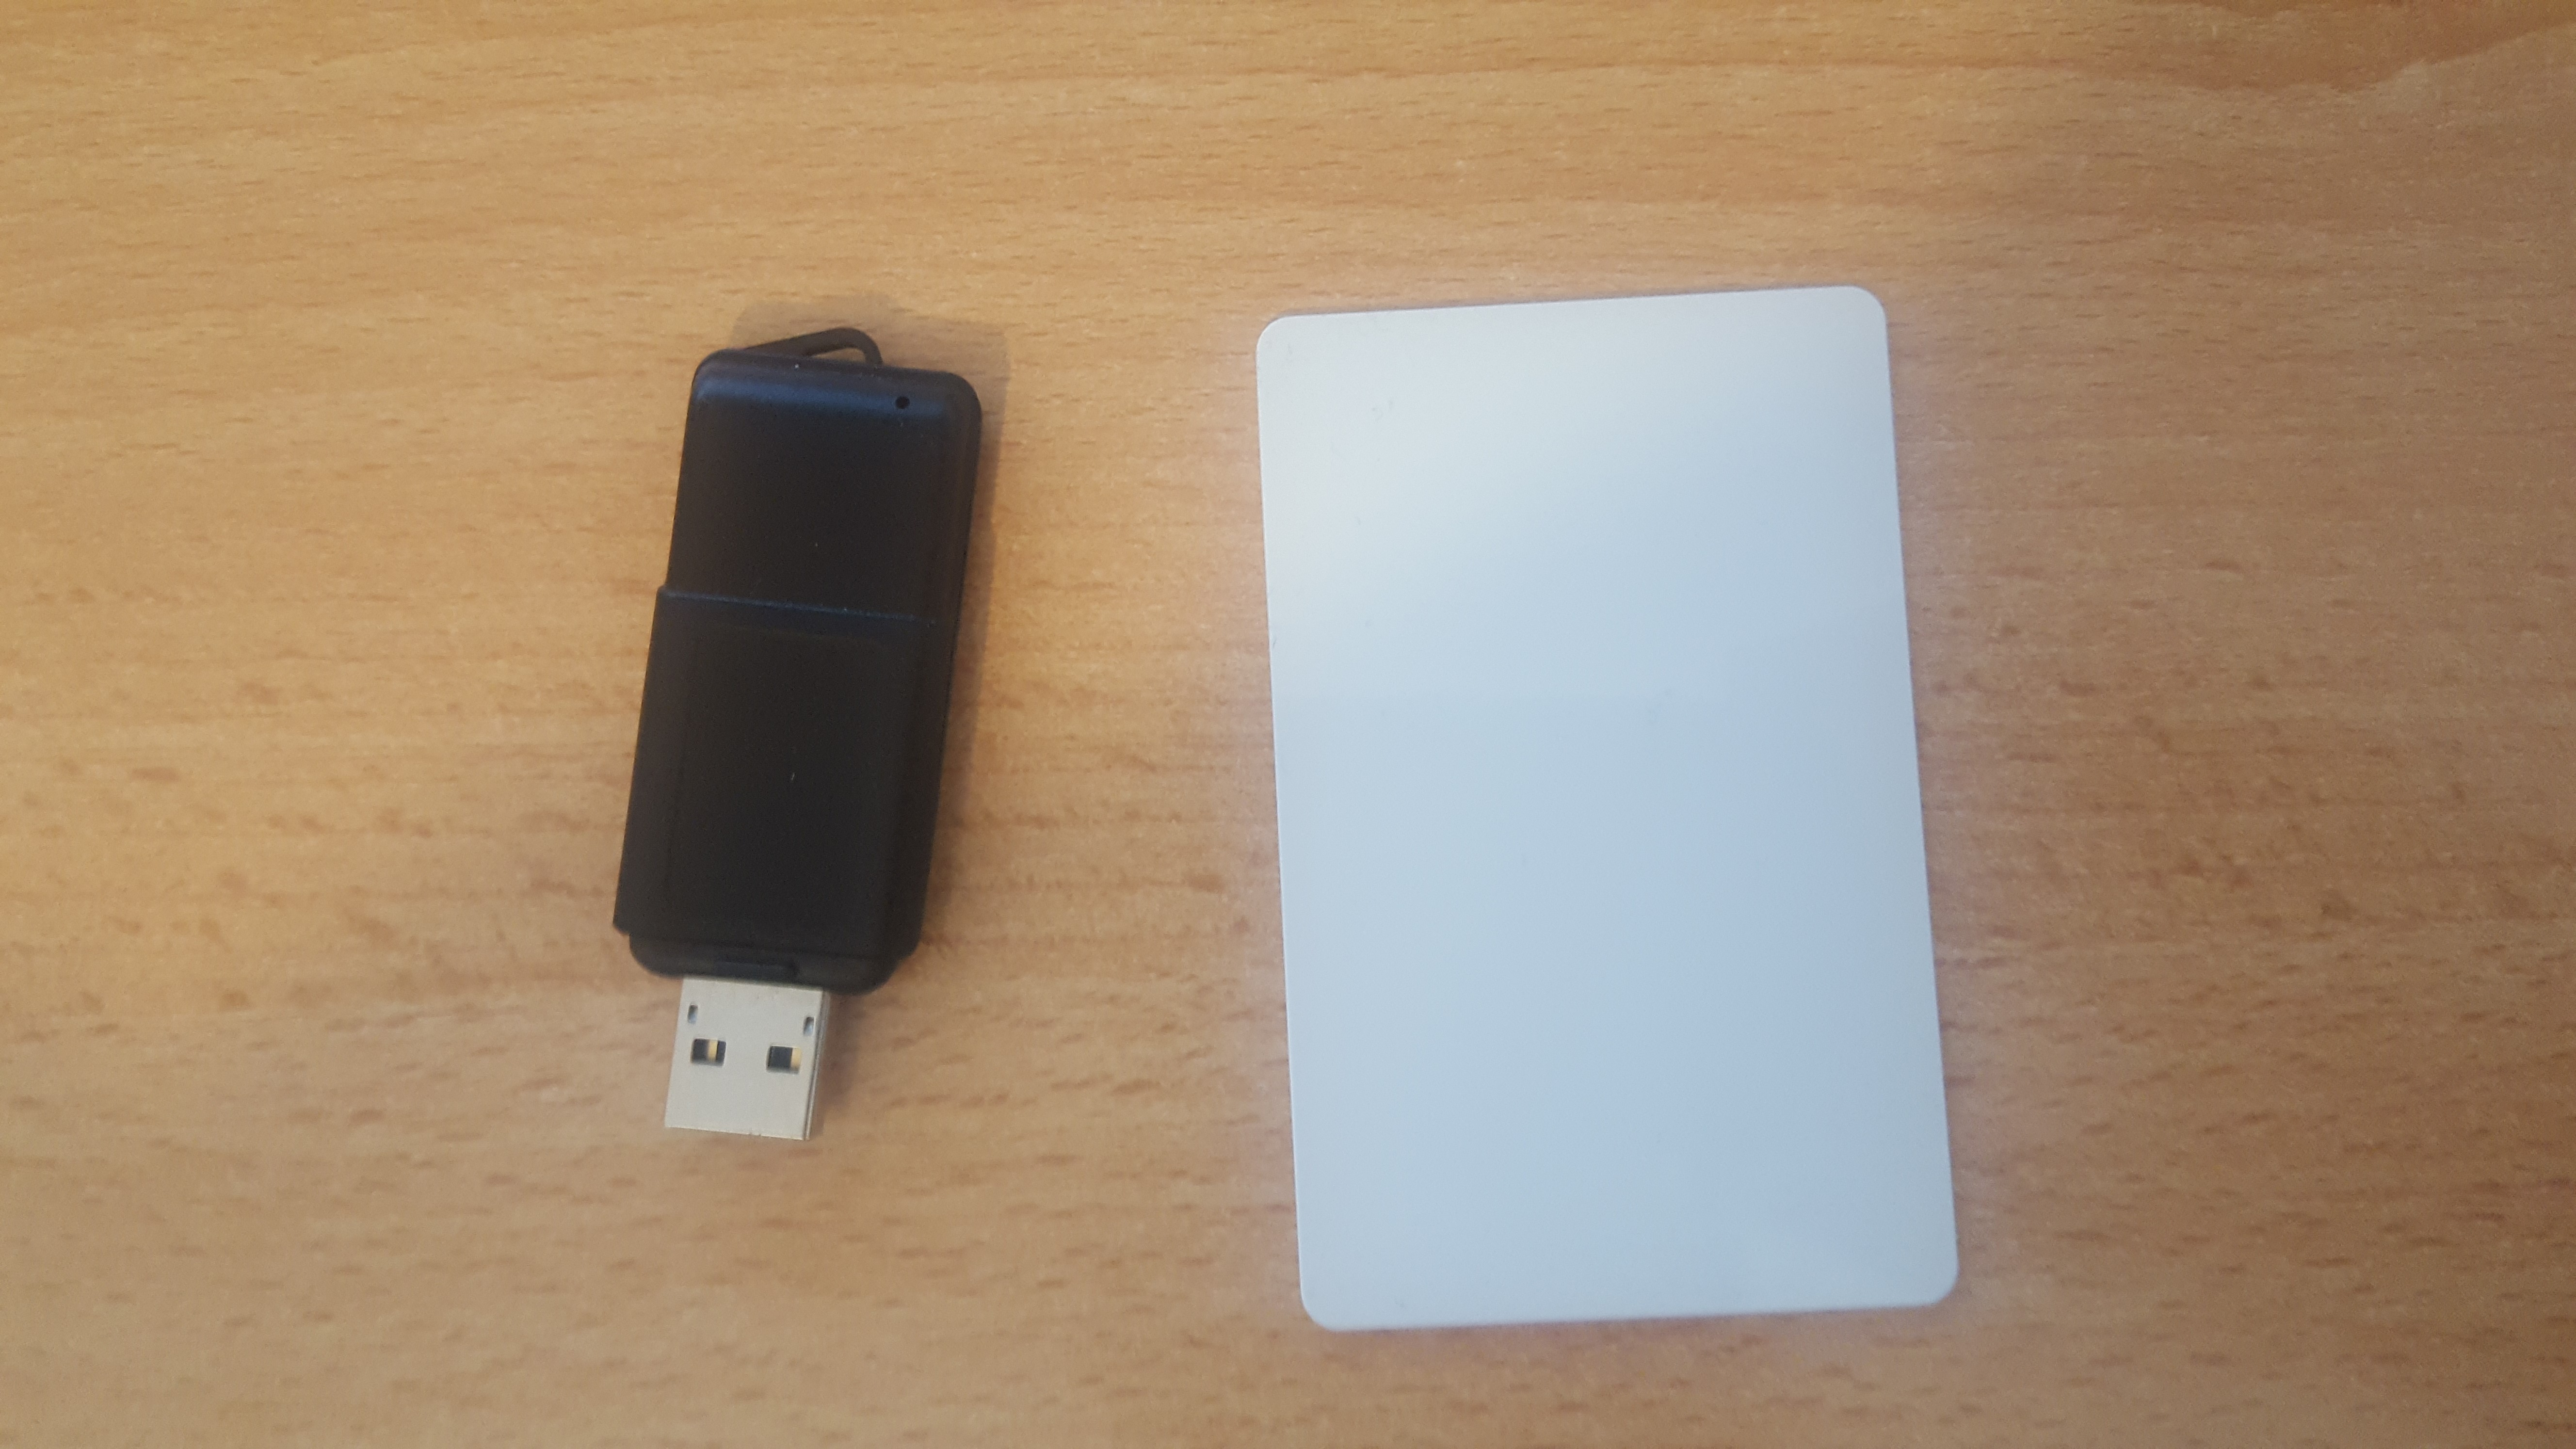
\includegraphics[scale=0.05]{introduction/hardware}
	\caption{Image of the USB card reader (right) and the smartcard (left) used in this project}
\end{figure}

When the appropriate Smartcard reader driver is installed in an operating system, the operating system can use an appropriate library to communicate with the smartcard via the reader.


Throughout the dissertation, a number of terms are used to refer to hardware used. They will now be defined, both in terms of actual hardware used in the project, and in terms of what they would refer to in a full-scale implementation of the proposed system:

\begin{itemize}
	\item \textbf{Card:} The Java Card used, referring to either the 2.2.2 or 3.0.4 card, depending on the context.
	
	\item \textbf{Reader:} The USB Smartcard reader shown in the image above. In general, this refers to the part of the system that communicates directly with smartcards.

	\item \textbf{Host:} The Windows PC on which the authentication software runs. In a realistic implementation, this would most likely be a low-powered and cheap device and operating system, perhaps a Raspberry Pi-tye device running a lightweight Linux distribution.
	
	\item \textbf{Terminal:} This term is used throughout the dissertation to refer to the combination of host and reader.
	
\end{itemize} 

\subsubsection{Java Cards}
Java Cards are programmable smartcards which allow for the programming of applets using a defined subset of the Java language and uploading those applets to the card. They enable secure storage of data using both persistent memory as well as a small amount of RAM, and support various cryptographic functions. 

As stated on the Oracle website: ``Java Card technology provides an architecture for open application development for smart cards, using the Java programming language".

Information on the development process for the Java Card platform can be found on page~\pageref{build_process}.

There are two approaches to Java Card development. “Masking” is when an applet is developed to be embedded into the card’s ROM during manufacture, alternatively an applet can be installed onto an existing card. The second method will be used for this project since it’s the easiest method for small-scale development and testing, however a for full organisation-wide rollout, masking may significantly reduce the aggregate manufacturing cost.



\subsection{Related Work}
TODO

Mention work done on Mifare and exposing weaknesses.

Any other implementation of asymmetric systems e.g. US government.

%Is this relevant? https://www2.ee.washington.edu/research/nsl/papers/ICAS-08b.pdf

%Does this have a similar result to my thing? https://link.springer.com/content/pdf/10.1007%2F978-3-642-12368-9_9.pdf

Cite paper on Opacity FS security, standards for various protocols.

Cite Denys' project from last year. Different approach, simpler more lightweight protocol.

Security Countermeasures for MIFARE Classic RFID cards - past project that summarises Mifare security.


\subsection{Project Outcome}
Overall, the project was successful, in that the success criteria have been met, and the project was completed broadly to the anticipated timetable. However, there was not sufficient time to implement any of the optional extensions suggested in the project proposal.

The primary difference between the initial project proposal and the course that the project took in reality was that in the project proposal it was suggested that there will be a full and proper comparison of available protocols. In practice, many alternative protocols were looked into briefly but it would have been difficult to  accurately assess any of them without a much lengthier investigation likely involving real implementations. There simply wasn't time.





%Preparation
\pagebreak
\section{Preparation}

\subsection{Starting point}
Prior to this project, I have had no experience with Java Cards, or smartcards in general. Most of my background knowledge in security comes from past Tripos courses, which in some cases briefly touch on material relevant to this course.

The main languages used in this project are the special Java subset used in Java Cards, and Python. Through my studies, I have gained good familiarity with Java, although the nuances of Java Card programming were previously unknown to me. I have also had a good amount of experience with Python from past work experience.

The code in the project is not developed from any pre-existing codebase but does make use of various libraries, detailed in section~\ref{subsec:libraries}, page~\ref{subsec:libraries}.


\subsection{Requirements analysis}
\label{sec:requirements}

In the project proposal, a number of success criteria were suggested. Here they are reiterated briefly discussed in terms of their context and how they might be addressed.

\begin{itemize}
	\item \textbf{The time taken for the reader to correctly authenticate the card should not exceed one second.}\\
	Smartcards have slow processing speeds, but the authentication process should be quick enough that it does not cause the user much inconvenience.
	
	\item \textbf{Access rights of a card should be revocable without having to modify the card itself.}\\
	This isn't possible with many existing systems which only rely on testing a card's knowledge of a secret key. In such systems, lost cards can continue being granted access as long as the system administrator hasn't had physical possession of the card to reprogram/destroy it. This criterion may be met by requiring cards somehow prove their unique identity, and blacklisting certain revoked cards.
	
	\item \textbf{The system should be sufficiently flexible to allow for an unlimited number of doors, each with different access privileges.}\\
	Asymmetric cryptography will allow a system to easily meet this criterion. Each card need only maintain its own key pair, so the storage requirements won't increase with the number of encountered card readers.
	
	\item \textbf{The system should be secure}\\
	To meet this criterion, it is important to consider all probable kinds of attack. Some research into the problems with MIFARE Classic and other common vulnerabilities can inform the process, and the final system should be subjected to a security evaluation.
	
	\item \textbf{The estimated large-scale introduction cost should not exceed the typical worst-case cost of a smartcard authentication system.}\\
	This criterion should be met as long as the proposed system doesn't prescribe additional expensive equipment beyond the smartcards themselves, the authentication terminals, and a card issuing system.
	
	
\end{itemize}



\subsection{Preparation strategy outline}
The development approach decided on for this project was the Waterfall model, because it fits the project much better then alternatives such as a spiral model or evolutionary model. This is because it is a relatively small project, completed by one person, within a limited time and with known requirements. It is most likely that, once some basic decisions have been made such as which protocol to implement, the first working prototype will be very close to the final project.

%TODO is this necessary?
Waterfall model steps:
\begin{itemize}
	\item \textbf{Requirements:} Already set out in the project proposal. 
%TODO: Should I include it and reference it?
	
	\item \textbf{Specification:} The process of refining the requirements to a more detailed specification is done in multiple parts. It is first touched upon in the requirements analysis section (page~\pageref{sec:requirements}), and further considered throughout the project when important decisions are made, such as the choice of protocol or authorisation method. %Could reference these sections
	
	\item \textbf{Implementation \& unit testing:} Implementation details are discussed throughout the Implementation section, with unit testing occurring throughout as described in the upcoming subsection, \ref{subsec:testing}.
	
	\item \textbf{Integration \& system testing:} All the individual components were used together without special code for testing individual functions. The nature of the task limited the amount of modularity available beyond the distinction between card and host code, so integration wasn't a big task. Testing consists of running the system as a whole using automatically generated values and some fixed test parameters.
\end{itemize}

It should be noted that the system is security-critical. This should be reflected in my implementation and testing strategy. For instance, the chance of data being stolen from any part of the system during online operation that may compromise the system has to be considered, and all possible points of weakness have to be considered. The system's security properties are assessed in the Security Analysis section, page~\pageref{sec:security_analysis}.

\subsubsection{Project structure}
The project will be split into modules that logically follow from the inherent divisions in the work. Card issuing and card authentication will be implemented separately, key algorithms will be separated into their own functions rather than integrated into large sections of code, and so on. 

Ease of modification is also a consideration. For instance, constants often occur multiple times in protocol implementations, so all the important constants are separated out into a separate class file.

\subsubsection{Testing}
\label{subsec:testing}

Testing and debugging can be performed on the host-side component of the system relatively easily, as with any other body of code.

Testing and subsequent debugging on the Java Card program is much more difficult due to the security-focused design that makes it impossible to obtain stack traces or variable prints, or follow code execution line-by-line, restricting feedback to a single response APDU for each command APDU.
 
As a result, testing and debugging could only be done as a series of separate executions, using breakpoints at various stages in the code and returning the relevant data, thus terminating the program. 
%Could mention simulations.

% TODO: describe system test.

% TODO: Get code snippet of this.


\subsection{ISO 7816}
Throughout the dissertation, I will reference certain things defined by the ISO 7816 smartcard standards. These in particular are things that I should clearly define.

%TODO applet

\subsubsection{Application Identifiers}
\label{subsec:aid}
An Application Identifier (AID) is a string of bytes that uniquely identifies an applet. Since the ISO 7816 standards permit multiple applets on each card, the AID is used to select specific applets on a card. 

The first 5 bytes of the AID is the Registered Application Provider Identifier (RID), the first byte of which is \verb|0xA_| for an international RID, or \verb|0xD_| for a national RID. An application provider can append up to another 11 bytes for the Proprietary Application Identifier Extension (PIX) to uniquely identify its different applications.


\subsubsection{APDUs}
An APDU, or Application Protocol Data unit, is the data format used in communication between the card reader and the smartcard. Communication occurs in command-response pairs in which the reader initiates an exchange with a ``command" APDU, and the card responds. The formats of these APDUs are defined in ISO 7816-4 \cite{TODO}.

APDUs facilitate stateless network-layer communication, analogous to HTTP, which results in a client-server model in which the card acts as the server. Any continuity between consecutive interactions between the reader and card must be implemented at a higher level, for example by including IDs in the data section of APDUs.

The following table is taken from the ISO 7816-4 part 5.1. It shows the actual structure of the APDU command-response pairs

\begin{figure} [ht]
	\centering
	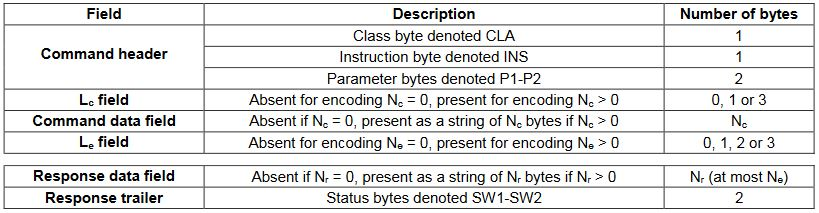
\includegraphics[scale=0.7]{introduction/apdus}
	\caption{Structure of Command and Response APDUs}
	From ISO 7816-4, Table 1 in section 5.1.
\end{figure}

Brief summary of the fields:

\begin{itemize}
	\item  Class byte -- type of command. bit 8 $b_8=0$ means interindustry class and the format is quite restricted. $b_8=1$ means proprietary class.
	
	\item Instruction byte -- indicates the specific command.
	
	\item Parameter bytes -- parameters for the instruction. In some cases, more convenient than using the data bytes.
	
	\item $L_c$ specifies how many bytes follow in the data field
	
	\item $L_e$ specifies the maximum number of data bytes that the smartcard is permitted to return to the reader.
	
	\item Command/Response Data field -- Arbitrary application-defined data.
	
	\item Status bytes -- Values returned to indicate whether the instruction was successful, or what error occurred. 0x9000 indicates that the instruction was executed by the card successfully. 
	%(TODO: explain other status words)
\end{itemize}


%TODO: Cover SELECT, other special APDU types



\subsection{Development Preparation}
Before work can begin on the main implementation, I need to invest time in ensuring that I fully understand the steps involved in the development process, that everything is set up correctly and that appropriate decisions are made regarding the structure of the project.

I used my Windows 10 PC throughout the development process, some details such as the backslash in path names may differ in other operating systems. I used the Atom text editor Atom to write code, since it can easily be configured with IDE plugins for multiple languages simultaneously, allowing for both the host-side and card-side application to be developed side-by-side.

The next step was to set up a remote backup and version control just to be safe, so I used GitHub to back up everything relevant to the project.

\subsubsection{Java Card 2.2.2 Build process}
\label{build_process}
Initially, I began development using the Java Card 2.2.2 platform. The following describes the process of developing applets for this version.

Setting up the development environment involved fixing a project structure and configuring environment variables according to the Java Card 2.2.2 Development Kit User's Guide \cite{jcdk_guide}, and installed \verb|api.jar| (enabling the use of Java Card functionality) and \verb|installer.jar| (to facilitate the installation process).

\textbf{Compiling:} The first step is compiling the code. The compilation of Java Card code uses the standard ``Javac" Java compiler, with \verb|api.jar| and \verb|installer.jar| included in the classpath. The source and output should be a version compatible with the Java Card version used. The \verb|-g| option to generate all debugging information is required for the converter step.
\begin{verbatim}
javac -g -source 1.5 -target 1.5 -cp ".\bin;
    ..\..\..\java_card_jdk\2.2.2\java_card_kit-2_2_2\lib\api.jar;
    ..\..\..\java_card_jdk\2.2.2\java_card_kit-2_2_2\lib\installer.jar" 
    -d .\bin src/uk/ac/cam/bo271/applets/opacity_zkm/*.java 
\end{verbatim}
The output is in the form of .class files.

\textbf{Converting:} The \verb|converter| is a binary included in the Java card Development Kit which converts the class files to a format compatible with Java Cards. This step first checks for any programming practices incompatible with the Java Card platform, such as the use of the `int' data type, or structural errors such as the lack of an applet class. The format for the command is as follows:
\begin{verbatim}
converter [options] <package_name> <package_aid> <major_version>.<minor_version>
\end{verbatim}

The package name (e.g. \verb|uk.ac.cam.bo271.applets.helloworld|) is the name of the package to be uploaded to the card. An AID, or Application Identifier, is a value allowing an applet to be uniquely identified (more details in section~\ref{subsec:aid}, page~\pageref{subsec:aid}). The Package AID is the AID of the entire package, not of a specific applet. Without specifying an applet AID, the package can only be used as a library by other applets. Specify an applet using the option 
\verb|-applet <AID> <class_name>|, where AID must have the package AID as its prefix.

\begin{verbatim}
call converter -exportpath 
     "..\..\..\java_card_jdk\2.2.2\java_card_kit-2_2_2\api_export_files;
     .\JCMathLib\bin" -classdir .\bin 
     -applet 0xD1:0xD2:0xD3:0xD4:0xD5:0xD6:0x01
     uk.ac.cam.bo271.applets.opacity_zkm.Opacity 
     uk.ac.cam.bo271.applets.opacity_zkm 0xD1:0xD2:0xD3:0xD4:0xD5:0xD6 1.0
\end{verbatim}

The output is a file in the form of a CAP (Converted APplet) file, with the \verb|.cap| extension, e.g. \verb|helloworld.cap|, which can then be uploaded onto the card. 

\subsubsection{Differences in Java Card 3.0.4 Build Process}
The installation process had to be revised midway through the project. This was due to the migration from java card 2.2.2 to 3.0.4 (see section~\ref{subsec:version_change}, page~\pageref{subsec:version_change}). The new process was different and had virtually no documentation, but I found an Apache ANT task which performs the compiling and converting stages. First a `build' file had to be produced in XML format, specifying the Java Card development kit path, the ANT task, AID, package etc. and making a call similar to:

\verb|ant -buildfile ant_tasks\build_opacity_opt.xml|

%TODO Stick example build file in appendix.
The output is also a \verb|.cap| file, but a different version.

\subsubsection{Uploading and running applets}
For both the versions described above, the upload process is almost identical. Once the applet is converted to a CAP file, it can be uploaded into the card using a GPShell script.

GPShell \cite{gpshell} is a scripting tool that implements the GlobalPlatform specifications \cite{globalplatform}, which determine the management of applets on a smartcard. It generates a series of APDU commands conforming to the GlobalPlatform specifications which upload the applet to the card.

In the following example GPShell script, the connection to the card via the reader is established, and the security domain applet is selected. This is what performs the applet management. For the GP211 specification, some card manufacturers set this as \verb|0xA000000151000000|, others use \verb|0xA000000003000000|.

A secure channel is then opened, any existing version of the applet deleted, and the .cap file is installed, and the connection is terminated.
\begin{verbatim}
mode_211
establish_context
card_connect
select -AID a000000151000000
#select -AID a000000003000000
open_sc -security 1 -keyind 0 -keyver 0 -mac_key 404142434445464748494a4b4c4d4e4f 
        -enc_key 404142434445464748494a4b4c4d4e4f
delete -AID C1C2C3C4C5C601
delete -AID C1C2C3C4C5C6
#install -file ..\code\applets\bin\uk\ac\cam\bo271\applets\challengeresponse
               \javacard\challengeresponse.cap -sdAID a000000003000000 -priv 2
install -file ..\code\applets\bin\uk\ac\cam\bo271\applets\challengeresponse
              \javacard\challengeresponse.cap -sdAID a000000151000000 -priv 2
card_disconnect
release_context
\end{verbatim}

%A full APDU trace for the upload script is available in TODO: appendix (also explain what APDUs do in the appendix section).

Other tools exist for uploading .cap files, such as the `apdutool' program supplied in the Java Card development kit, but I found GPShell was more flexible and usable.

\subsubsection{Practice}
Before starting work, I had to gain familiarity with the aforementioned tools and processes, and find the best approach.

First, used GPShell and a pre-compiled test applet in .cap format that came with it to write a test script to upload the applet, list contents, and  uninstall it.

Then I attempted to run an applet using host-side code. Initially I attempted to use OpenCard Framework, but had to switch to an appropriate Python library (section~\ref{subsec:python_pcsc}, page~\pageref{subsec:python_pcsc}), which worked for the simple ``hello world" applet.

The Java Card development kit comes with some source code for sample applets that demonstrate applet structure. I used these to test the compilation and conversion steps, and then uploaded a simple one to the card to ensure everything worked properly. I had some initial problems due to using the incorrect JCDK version which was incompatible with the cards, but it worked eventually.

The next step was to write a simple command-response test applet that stored an input string, and returned it later. In this step, I learned about the various quirks and limitations the Java Card library and platform (e.g. int-to-short casting, restrictions on APDU passing, different garbage collection system). This took quite some time as online resources for Java Card development is scarce.

At that point I judged that I had learned the development procedure well enough to begin development of the main applet. It was then easy to combine all the main steps; compiling, converting, uploading and running, into shell scripts that allow new builds to be executed with minimal effort. An example script for the Java Card 3.0.4 build is as follows:
\begin{verbatim}
call ant -buildfile ant_tasks\build_cr.xml
GPShell.exe gpshellscripts\crinstall.txt
python ..\code\Python\Challengeresponsehost\ChallengeResponse.py
\end{verbatim}

\subsection{Host to Card interface}
To develop applications that run on some conventional Windows/Linux operating system which can communicate with a contactless smart card, I not only needed a suitable card reader, but also suitable libraries that provide access to the functionality of the reader.

\subsubsection{OpenCard Framework}
Initially, the OpenCard Framework \cite{ocf} was identified as a potential Java-based middleware/API that could be used for developing the host-side part of the project. It was developed many years by the OpenCard Consortium and mostly driven by IBM.

However, upon writing some code for a sample project and attempting unsuccessfully to run it, I noted that the framework was failing to recognise the card reader.

after much frustration, I discovered that the OpenCard framework must be explicitly implemented by the smartcard reader for the middleware to work. Many commercially available readers, including  the one used in this project, do not support it, and instead only support the more common PC/SC framework. My initial assumption had been that OpenCard was a wrapper for PC/SC, but this was disproven by the fact that some reader data sheets specify PC/SC and OpenCard whereas others only specify PC/SC.
%Could back up claim that only some cards support OCF

\subsubsection{PC/SC}
After the failed attempt at using the OpenCard framework, it was clear that PC/SC was required. 

PC/SC \cite{pcsc} is a standard API that interfaces smartcards and smartcard readers with a PC. Windows comes with a PC/SC implementation by default, while there exists a less complete but perfectly functional implementation for Linux and Mac OSX, called PC/SC-lite. 

The PC/SC API is implemented in C, though various bridges/wrappers exist for other languages. Not all languages have a library for PC/SC support, but many do, including Java, Visual Basic, and Python.





%Implementation
\pagebreak
\section{Implementation}
%Could add more things in here relating to learning dev process.

\subsection{Chosen Protocol - opacity ZKM}
%TODO: Reference the other protocols looked at, mention that they were briefly examined and Opacity ZKM seemed to fit the requirements best.



The Opacity protocol standard defines two protocols; Opacity ZKM (Zero key Management) and Opacity FS (Full Secrecy). The main difference between the two is in the authentication of the terminal. Opacity ZKM doesn't require the terminal contain any secrets and therefore cannot be authenticated by the card, whereas Opacity FS requires terminals have certificates much like cards, which can be authenticated by the card.

During the development process, I looked at two versions of the Opacity specification. The first, which distinguished between the basic and optimised protocol, was a freely available but slightly outdated document \cite{opacityfree}. The second was an official ANSI document \cite{opacity} which only described the protocol with the Persistent Binding  optimisation. It addressed many ambiguities in the older protocols, with only some very minor semantic differences, which were taken into account, though these aren't really worth covering at length. It also fixes some errors, such as those described in section \ref{subsec:pb_errors}, page \pageref{subsec:pb_errors}.

\subsubsection{Brief overview}
A simplified overview of the primary steps of the Opacity ZKM protocol are as follows:

\begin{enumerate}
	\item Cards issued with certificates signed by root key
	\item Terminal generates an ephemeral (one-time use) key pair for the interaction.
	\item Both sides perform ECDH, use the result to derive session key
	\item Use session key to generate a Message Authentication Code using CMAC for session-specific data, proving the card knows the private key corresponding to its certificate.
	\item Card sends the nonce, MAC, and certificate to the terminal
	\item Terminal uses the root public key to verify the certificate, and checks the MAC value.
\end{enumerate}

%Describe auxiliary protocols
\subsubsection{Elliptic Curve Cryptography}
Elliptic Curve cryptography is a form of asymmetric cryptography based on elliptic curves of the form $y^2=x^3+ax+b$ over finite fields. 
\begin{figure} [ht]
	\centering
	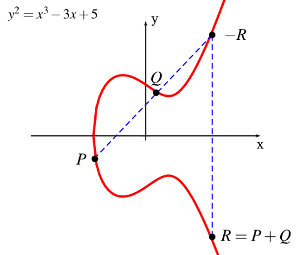
\includegraphics[scale=0.5]{implementation/elliptic_curve}
	\caption{Illustration of elliptic-curve point addition}
	Taken from a Stackoverflow page \cite{ec_diagram}, via Google Image Search.
	\label{figure:ec_add}
\end{figure}

The operations used in EC cryptography are Elliptic Curve addition and multiplication, which differ from regular addition and multiplication significantly, but still have the desired properties for repeated additions of some initial ``generator" point form a cyclic group. Addition of two points consists of finding the third intersection of the line between them and the curve, and reflecting in the $x$-axis to find the result $R$ (as shown in figure \ref{figure:ec_add}). EC point multiplication with a scalar $k$ is the result of $k$ repeated additions of the point with itself.

Given a generator $G$ and some private key $d$, the corresponding public key is the result of the EC point multiplication, $Q=d \cdot G$. It is computationally infeasible, given some $Q$, to find the corresponding $d$, so the scheme is secure.

Elliptic Curve cryptography requires keys of a smaller length than other forms of asymmetric cryptography to achieve the same level of security, so is sensible in a smartcard application where resources are limited.

The specific curve used in the Opacity specification is the NIST P-256 curve \cite{p256}. Given that it was developed by the U.S. government, there has been some speculation as to whether there may be a secret ``backdoor" that allows it to be broken, though there is no evidence for this.

In the Opacity ZKM protocol, it is used for generating session keys via Elliptic Curve Diffie-Hellman (section \ref{subsec:diffie_hellman}) and for generating certificate signatures and verifying them via ECDSA (section \ref{subsec:ecdsa})


\subsubsection{ECDSA}
\label{subsec:ecdsa}
ECDSA, or Elliptic Curve Digital Signature Algorithm, is a version of the Digital Signature Algorithm (DSA) using Elliptic Curve cryptography.

A Digital Signature is a construct in public-key cryptography for proving the authenticity of the source of some information. The owner of a key pair ``signs" some information using their private key, and any other party can verify that the signature was produced by the keypair owner using the corresponding public key. 

%Could explain further how ECDSA works if more content needed.

The purpose of its use in the Opacity ZKM protocol is to verify the authenticity of the CVC certificates issued to the terminal by the key issuing authority. During the authentication process, the terminal uses the issuing authority's public key(s) to verify that the certificate is genuine, proving that the public key used by the card and included in the certificate corresponds is one that was validated by the certificate issuing authority.

\subsubsection{ASN1}
ASN.1, or Abstract Syntax Notation 1, is a standard for data encoding. There are multiple ways it can be used, and the ASN.1 format used in Opacity is the BER (Basic Encoding Rules) format, which is primarily used for formatting and parsing the certificate. 

Values are encoded in ``TLV" form (Type-Length-Value). Complex data formats can be achieved by combining primitive and constructed data types, for example using the ``sequence" type which consists of a sequence of other TLV values.

\begin{figure} [ht]
	\centering
	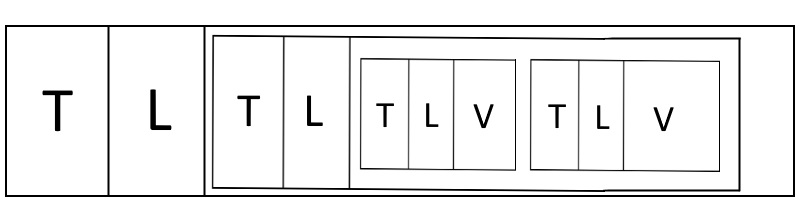
\includegraphics[scale=0.7]{implementation/tlv}
	\caption{Illustration of the BER ``TLV" structure}
\end{figure}

During the card issuing stage, a new certificate has to be created. It makes far more sense for this to be done by the issuing host device, rather than the card, since it can be done much faster and the host must generate the signature for the certificate in any case.



\subsubsection{Elliptic-Curve Diffie Hellman key exchange}
\label{subsec:diffie_hellman}

\textbf{Key exchange }(or key establishment) is any process by which cryptographic keys are exchanged between two parties to enable cryptographic methods, particularly encryption/decryption, to be used in communication between the parties.

The \textbf{Diffie-Hellman Key Exchange} is a simple asymmetric cryptographic key exchange protocol, enabling two parties to negotiate a shared secret value across an insecure medium which no eavesdropper can reproduce.

In the most general case, there is some known cyclic group $\mathbb{G}$ and a generator $g$ for the group. These can be public. A has a secret key $x \in \mathbb{G}$, B has a secret key $y \in \mathbb{G}$. A computes $g^x$ and sends to B, and B computes $g^y$ and sends to A. A and B can then take the received value to the power of their own secret key, calculating $g^{xy}=g^{yx}$. This value is the shared secret.

Secrecy is ensured due to the \textbf{Discrete Logarithm Problem}, which states that it is computationally infeasible for anyone with access to any $g^s$ to calculate $s$ (and in fact, there may be many solutions to the discrete logarithm, only one of which is the original power). An eavesdropper therefore cannot calculate the shared secret $g^{xy}$ from knowledge of $g^x$ and $g^y$ for this reason.

The \textbf{Elliptic-Curve Diffie Hellman} (EC-DH) protocol is one kind of implementation of the Diffie-Hellman key exchange method using Elliptic Curve cryptography. The shared secret is the X-coordinate of the result of the point-multiplication of one party's private (scalar) key and the other's public (point) key.

In the Opacity ZKM protocol, the EC-DH step is one of the first actions performed by the card and terminal, using the card's persistent keypair and the host's ephemeral keypair to establish a shared secret which is the basis for further steps. 

By executing this step, the card must know the private key corresponding to the public key contained in its certificate, which is signed by the root key. Therefore, the fact that the card successfully executes this step and obtains a shared secret with the host proves that it is the intended owner of the certificate (assuming secret keys have not been stolen). This fact is demonstrated to the host later on during the C-MAC step (section \ref{subsec:cmac}).

The EC-DH step is not executed in subsequent interactions under the Persistent Binding optimisation (section \ref{subsec:pb}, page \pageref{subsec:pb}), however the shared secret used in these interactions originally derives from the EC-DH step in the first interaction, so it is still secure.



\subsubsection{Key derivation}
\label{subsec:kdf}

The key derivation function (KDF) is used to derive a set of session keys, as well as next time's shared secret if the persistent binding optimisation is used, from this session's shared secret $Z$. The KDF used in the Opacity protocol is defined in the NIST SP 800-56A standard, section 5.8.1 \cite{TODO}. It involves creating an (almost) arbitrarily long sequence of pseudo-random bytes by repeatedly taking the hash of $Z$ with some session-specific `info' data, incorporating randomly generated session-specific data from both the card and terminal, ensuring the only way to correctly acquire the key material is by knowing $Z$ (and not, for instance, reusing data from another interaction). The KDF is defined as follows:
\begin{align*}
\text{DerivedKeyMaterial} =\ &\text{hash}(0\text{x}00000001||Z||\text{info})||\\
&\text{hash}(0\text{x}00000002||Z||\text{info})|| \cdots\\
&\text{hash}(0\text{x}00000000+n||Z||\text{info})\\
\end{align*}
This function is used to derive 96B of keying material; $\mathsf{SK}_\mathsf{CFRM}||\mathsf{SK}_\mathsf{MAC}||\mathsf{SK}_\mathsf{ENC}||\mathsf{SK}_\mathsf{RMAC}||\mathsf{NextZ}$. $\mathsf{SK}_\mathsf{CFRM}$ is used to generate the C-MAC, and $\mathsf{SK}_\mathsf{MAC}$, $\mathsf{SK}_\mathsf{ENC}$ and $\mathsf{SK}_\mathsf{RMAC}$ are optionally used to facilitate any further system-specific interaction between the terminal and card, though this should be treated with caution due to the false terminal attack, described in the security analysis section, \ref{sec:security_analysis}, page \pageref{sec:security_analysis}.


\subsubsection{CMAC}
\label{subsec:cmac}
C-MAC is a Cipher-based Message Authentication Code (MAC) generation algorithm, used to generate codes that prove a message was sent by someone with a specific key. An explanation of the algorithm is given in appendix \ref{cmac_expl}. There, I explain that the advantage of C-MAC over its predecessor CBC-MAC is in security for variable-length inputs, however the C-MAC inputs used in Opacity ZKM are fixed-length at 38B. Regardless, this is fine since the use of C-MAC has no inherent disadvantages. However, there were complications in that the Java Card versions used lack support for C-MAC, so it had to be implemented manually.

The purpose of the C-MAC step in the Opacity ZKM protocol is for the card to prove that it shares the same session key as the host. The key derivation inputs are different each time and hence so is the session key, and the C-MAC inputs include host and card IDs, and ephemeral host public key (which is different each time), meaning the C-MAC inputs are different each time and only applies to the specific session. 

The card proves by executing and returning the C-MAC for these inputs that it derived the same session key $\text{SK}_{\text{CFRM}}$ as the terminal. This implies that the card completed the key derivation step successfully, which in turn implies that the card shares the secret with the host, which comes from either an EC-DH step, or from a previous interaction via the Persistent Binding optimisation  (section~\ref{subsec:pb}, page~\pageref{subsec:pb}) which was originally acquired from another EC-DH step.

This fact that the card can only have computed the C-MAC correctly if it was able to complete the EC-DH step (when brute-force attacks are discounted as infeasible) proves its authenticity, as explained in section \ref{subsec:diffie_hellman}.

%Could describe why MAC is preferable to a signature. Easier to compute?


%outline program structure with code snippets
\subsection{Java Card Protocol Implementation}
%First: outline basic features of javacard application. (could be moved to preparation section)

%Give good code abstractions, explain overall design decisions. 

This section describes the base implementation. For details about optimisations, see section~\ref{sec:optimisations}, page~\pageref{sec:optimisations}.

\subsubsection{Program structure}
%Could Move to Preparation Java Card section depending on word counts.

All Java Card applets must adhere to a basic program structure, which is modelled by extending the abstract ``Applet" class and implementing the methods included in it. Only classes extending the Applet Java Card library class can be directly interacted with when uploaded onto the card, though other classes may be included in the package and used by the applet class. The primary methods that should be implemented are \verb|install()|, and \verb|process(APDU apdu)|, though other methods may optionally also be implemented.

The static \verb|install()| method called when applet is first installed. It should create a new instance of the applet class, in my case by executing \verb|Opacity applet = new Opacity();|. It should then call the \verb|register()| method on the new applet instance (TODO: why?). Either the \verb|install()| method, or the applet's constructor, should initialise the state of the applet and create persistent objects in EEPROM which are to be used in later interaction.

The \verb|process(APDU apdu)| method is the point of entry into the applet for typical runtime use, executed when that applet is currently selected and a new APDU is received from the terminal, where the APDU is encoded into a Java Card ``APDU" object and given as the argument. The \verb|process()| method takes an appropriate course of information based on the information contained within the APDU. My implementation ensures the class code is 0x80 (user-defined), and executes a switch-case statement on the instruction code. A subsidiary function is then called depending on the instruction code. This allows modularity at the level of high-level functions, and easy modification of supported functionality.

%TODO: include code snippets. 

%Could discuss limitations in how APDU is passed, lack of int type, standard libraries inaccessible, different libraries exist etc

%\subsubsection{Memory management}
%Outline different types of memory, how they're allocated.

%Mention what things should be persistent or transient. Absolutely necessary that recurring things should be persistent. Reference parts of Opacity protocol that require this e.g. certificate, key pair. Persistent ID prevents recomputation etc.

\subsubsection{Java Card C-MAC Implementation}
\label{cmac_impl}

%TODO reference appendix source code.

There was no library C-MAC functionality in either Java Card version I attempted to use (2.2.2 or 3.0.4). It was only introduced in 3.0.5 (reference cards not yet available). Consequently, I had to write my own implementation to fulfil the role described in section \ref{subsec:cmac}. 

I deemed it best to write an implementation that can be used in virtually the exact same way as if it were a library implemetation, so I wrote a class AESCMAC128 which extends Signature (the abstract class for digital signatures). The instance would be created in the Opacity class constructor and stored in EEPROM. It would make use of transient byte arrays because operations would not need to be performed across multiple accesses.

On the Java Card 2.2.2 platform, I used the \verb|ALG_AES_MAC_128_NOPAD| mode of the Signature class as an auxiliary function in the C-MAC algorithm. For unknown reasons, this option didn't work in the version 3.0.4 cards I had acquired, so instead I made use of the structural similarity to CBC-MAC, using the \verb|ALG_AES_BLOCK_128_CBC_NOPAD| mode of the Cipher class. Both of these approaches worked well.

%TODO: Maybe more in-depth implementation details.

\subsubsection{Java Card EC-DH Implementation}
With the Java Card 2.2.2 version, the library implementation of ECDH proved to be a big problem. Ordinarily, the shared secret outputted by ECDH using 256b elliptic curves would be the 32B result of the point-multiplication operation with one party's private key and the other party's public key. However, in the Java Card 2.2.2 implementation, it only returned the 20B SHA-1 hash of this value, causing much confusion.

This was useless in implementing the Opacity protocol, since the shared secret is required in its raw form as an input to the key derivation function (section~\ref{subsec:kdf}, page~\pageref{subsec:kdf}).

Initially I attempted to implement elliptic-curve point multiplication manually, though as described in section~\ref{subsec:version_change}, this attempt failed, forcing the move to the Java Card 3.0.4 platform, which supported returning the raw ECDH value rather than the hash.

\subsection{Host-side Implementation}

The choice of language for the host-side implementation was motivated far more by language preference than by necessity. Python has the library `pyscard' (PYthon Smart CARD), developed by Gemalto, which interfaces with both PC/SC on Windows and PC/SC Lite for Linux/OSX, allowing my code to access the USB card reader.

%TODO much of this is more suited to the evaluation.
Both Python and the library are highly portable, meaning I could develop on Windows in the knowledge that the code could easily be ported to most other operating systems and devices, making it a good choice. Another motivation was that Python is well suited to flexible development, since I started with no experience of smartcard development and knew I would need to be able to make lots of changes and constantly test things. I had lots of experience with Python to begin with, so it was also convenient not to have to learn a new language.

In my prototype implementation, information required by the terminal such as the root public key was simply stored in the file system and accessed by the program when needed. A proper system would likely use a slightly different approach but the principle is the same, so it makes sense in a prototype.


%TODO: include code snippet




\subsection{Certificate issuing}
The certificate issuing process isn't specifically defined in the OPACITY specification, only describes how cards are authenticated, i.e. how a terminal ensures a card was issued by a valid issuing authority and hasn't been revoked. Other details such as how cards are issued, and later a terminal establishes whether or not a legitimate card has permission to access it, are left to the implementer.

To authenticate a certificate, each terminal must be programmed with the public key counterparts corresponding to any private keys used by the issuing authority to sign certificates, enabling the terminal to verify the signature in the certificate presented by the card. Multiple signers of CVCs are supported by Opacity. In section 9.2, annex C of the free protocol documentation \cite{opacityfree}, it recommends that, in this case, the rightmost bytes of the Issuer Identification Number in the CVC should reference a particular verification public key. For my prototype I only used one issuing keypair, though extending this to many keypairs would be simple.

In a realistic system, one issuing authority should be able to issue cards with varying access control permissions. The rest of this section will discuss how this will be achieved.


\subsubsection{Certificate structure}
The certificate format used for Opacity certificates is the Card Verifiable Credential (CVC) format (see appendix \ref{cvc}, page \pageref{cvc}). This contains the following fields:

\begin{itemize}
	\item \textbf{Credential Profile Identifier:} value that denotes the protocol version used. This value is set to 0x80 for this protocol version.
	
	\item \textbf{Issuer Identification Number:} 8B value. IssuerID (6B) $||$ IssuerKeyID (2B). IssuerID denotes the issuer and is the leftmost 6B of the hash of the unique issuer name. 
	
	\item \textbf{Globally Unique Identifier (GUID):} 16B unique application-specific value that identifies the specific card.
	
	\item \textbf{CardHolderPublicKey:} Public key for the card's Elliptic Curve key pair, unique to that card and generated by the card. Encoded along with the ASN.1 object identifier for the elliptic curve used to generate the key pair. For this implementation, the object identifier is that corresponding to the NIST P-256 curve, 1.2.840.10045.3.1.7.
	
	\item \textbf{DigitalSignature:} The signature for this certificate, using ECDSA with sha-256 with the certificate issuer's key. The information included in the signature is not explicitly defined in the Opacity standard, but certificate signatures are typically generated from other important parts of the certificate. In my implementation, I generated the signature from the concatenation of the Issuer Identification Number, the GUID, the ASN.1-formatted public key, and the RoleIdentifier.
	%TODO double check that signed info not explicitly defined.
	
	\item \textbf{RoleIdentifier:} 1B code identifying the role that this certificate holds. The CVC certificate structure is used in different situations. Root certificates, assigned to the keypair that signs cardholder certificates, have their own role identifier which is 0x12 if the root application is a card application, and 0x22 if the root application runs on a client.
	
	The vast majority of certificates will of course be cardholder certificates, assigned to each card. The corresponding role identifiers that may be used in the Opacity ZKM protocol are 0x00 for typical cards, and 0x80 for administrator cards. 
\end{itemize}

\subsubsection{Certificate generation}
\label{subsec:certificates}

The certificate issuing process is performed at the beginning of the lifetime of each card, and is the process in which the card is first issued the certificate that it will use in all future authentication attempts.

The process, as implemented, is carried out as follows:
\begin{itemize}
	\item The Issuing authority, modelled by the Python file \verb|Issuer.py|, loads the root private key. In the prototype, this is modelled by simply loading the unencrypted value from a file. This isn't a secure approach and a full implementation would separate the issuing device from all other networks and systems, mitigating the chance of theft of the key. %TODO is this last point repeated?
	
	\item The issuing authority then selects the Opacity applet in the smartcard, and calls a method on the card \verb|init_keys(apdu)|, causing it to generate and save its SecP256r1 (NIST P-256) Elliptic Curve key pair, and return its newly generated public key.
	
	\item It then formats and generates the certificate, signed by the root key using ECDSA. Ideally, specialist hardware would be used to store the key securely, and sign data without ever needing to return the key.	
	
	\item The certificate is then uploaded to the card, which saves it for future authentication.
\end{itemize}


\subsection{Authorisation Options}
The Opacity ZKM protocol encompasses how a card terminal can authenticate a card i.e. can verify that the card's certificate was originally issued by the certificate issuing authority governing that particular terminal. 

This is a good start, however in general, an access control system has multiple terminals, all of which should support different access control restrictions, for instance based on role or department. Furthermore, it should be possible to manually reconfigure the access control system without requiring physical access to individual cards. Once authentication has been completed, the process of determining what access should be granted to a card is called \textbf{authorisation}.

Importantly, the authorisation method chosen should be cryptographically secure, and not permit any kinds of attacks that would allow an attacker to gain any access that they should not have.

Clearly the authorisation process should take place entirely on the terminal (based on verifiable information provided by the card), since the card should not be trusted to be honest about its permissions.

I will look at a number of different approaches and judge them based on flexibility, security and convenience, and will make the assumption that terminals aren't connected to a secure network, since this is impractical in many cases.

\subsubsection{Multiple root keys and Issuer Identification Numbers}
%TODO: describe how IINs are involved in this. IIN can be used to identify which key was used to sign each certificate without the terminal having to attempt signature verification for each public key it recognises.

One approach would be to have multiple root keys (each with their own IIN) for certificate issuing, with each terminal programmed to accept certificates with a certain key or one of a set of keys.

Each card should still only have one certificate, since multiple certificates would require significant deviation from the Opacity ZKM protocol and may exceed the memory available on smartcards. Both of these things violate the goals of this project.

Using this as the only access control mechanism essentially means there would have to be separate root keys for each possible role in the organisation, with terminals configured with the root public keys to validate certificates corresponding to a list of allowed roles.

The amount of fine-grained modification this allows is limited. Without physical access to cards to reconfigure them, a system administrator can only blacklist cards from terminals (supporting card revocation and permission denial), but whitelists are impossible since terminals don't have the means to validate certificates whose issuing key it doesn't recognise.

It may also be easy to misconfigure terminals since the system administrator must choose the correct subset of a long list of roles to allow for each terminal, which can easily go wrong.

This approach is reasonable but not ideal. It may be included as an option to be used in conjunction with another access control method.

\subsubsection{GUID}
The Globally Unique Identifier (GUID) is a 16B value that is unique to a card, or possibly a cardholder (if, for example, spare cards are allowed). GUIDs are included in the information used to generate the certificate's signature, so a card cannot falsify its GUID to gain additional access. Terminals could be configured to use this value to determine a card's permissions.

There are two broad possibilities for this approach:
\begin{itemize}
	\item When certificates are issued, GUIDs are chosen completely at random or by some counter. The value itself would have no semantic meaning, so access control is enforced by terminals which either allow any GUID not on a blacklist, or only allow valid GUIDs on a whitelist.
	
	This system would require a lot of maintenence, since each time a new card added to the system the relevant terminals have to be configured accordingly.
	
	\item Part of the GUID could be reserved to encode permissions, such as the first 8B, with each bit representing access to a particular terminal/department. The other 8B is unique, perhaps encoding some existing identifier (e.g. the Cambridge University CRSID, or some card identifier).
	
	This would have the advantage that terminals wouldn't store much explicit access control data, and wouldn't need to be updated for newly issued cards. Blacklists and whitelists can be used to make finer adjustments to access control, including but not limited to revocation.
	
	Reconfiguration of terminals is possible by altering the accepted GUID strings, but this is constrained in some cases. For example, if a single bit represents access to two doors A and B but the administrator wants to separate them, the only way to do this without recalling all cards is with massive changes to their whitelists and blacklists.
	
	Another slight disadvantage is privacy. When a card gives its certificate, eavesdroppers can quickly determine what access the card gives. Even if GUID encryption is used, a false terminal can trick a card into releasing it. This may be used by an attacker to identify potential targets for theft.
\end{itemize}

Security properties are good overall, since any changes an attacker makes to the GUID will cause the digital signature validation to fail.


\subsubsection{Card ID}
Discriminate based on card ID. Card ID is first 8B of the hash of the card's CVC certificate, and terminals could be supplied with a whitelist of card IDs they should allow, or a blacklist of card IDs they should deny.

There are $O(2^{64})$ possible values, so according to the Birthday problem \cite{birthday}, there would have to be approximately five billion cards for a 50\% chance of two cards having the same ID. This is acceptable, so it is feasible to use card IDs to discriminate between cards. It's also infeasible for an attacker to brute-force generate certificates to find one with a desired ID, but even if it weren't, the issuing authority is unlikely to allow the attacker that many attempts. Attempting to generate a certificate whose ID matches at least one other in existence is infeasible in all but the largest systems.

The main disadvantage is the fundamentally unstructured nature of hashes, meaning card IDs can't encode access control data (unlike the GUID). Therefore, this only works if whitelists/blacklists are updated on relevant terminals for each new card.

\subsubsection{Public Key}
Terminals could discriminate based on the card's public key. Since public keys can only be derived from randomly chosen private keys, the only way to find public keys with desired properties is by brute-force search \cite{facebook_onion}, which is impractical, certainly if the smartcard is generating its own key pair. Therefore the public key won't be used to encode access control data. The only alternative, much like with the card ID, is to rely entirely on whitelists and blacklists.

A public key is covered by the signature in the certificate, proving it belongs to an authorised card. Due to the nature of asymmetric cryptography, it's computationally infeasible to pass authentication using a false public key, so this approach is secure. The 256b public key is more secure from brute-force attacks than the 64b card ID, though both cases are adequate.


\subsubsection{Authorisation implementation}
Authorisation is carried out entirely by the terminal, so different terminals can use different methods, but here I will describe the recommended approach, used in the prototype.

I judged the approach of encoding access control data in the GUID to be the best start since it limits the necessity for a system administrator to reprogram terminals to exceptional circumstances.

The slight privacy disadvantage due to cards effectively advertising their permissions is a concern, and virtually impossible to eliminate without a means to authenticate terminals (which violates the requirement that terminals do not store secrets).

The final implementation involves configuring each terminal with a GUID mask value which is XORed with a card's GUID, and the terminal grants access to the card if the result is non-zero. This is a simple approach, minimising the possibility of error, and quite adaptable; each of the 64 bits can represent a single door for a small organisation, or an entire department/role for a larger organisation, however there are clearly limits to how much it can scale without sacrificing fine-grained control. Use of multiple root keys is also possible under this system if so desired.

\subsection{Optimisations}
\label{sec:optimisations}
\subsubsection{Persistent Binding}
\label{subsec:pb}
%TODO could put optimised timeline in appendix and link it

The Opacity protocol describes the Persistent Binding (PB) optimisation. Without the optimisation, a card and terminal must perform Elliptic-Curve Diffie-Hellman key agreement upon each encounter to establish a shared secret. 

The optimisation allows the terminal and card to cheaply generate a shared secret from key material derived from the Key Derivation Function that is used in subsequent interactions. The shared secret is then stored by both sides and indexed by the ID of the other party for subsequent lookup.

In the implementation of PB, I used an XML file to represent the host-side PB store, and a linked list to store PB entries on the card.

\subsubsection{Errors in Persistent Binding specification}
\label{subsec:pb_errors}
During implementation, I identified a couple of errors in the description of the optimised ZKM protocol, page 40 of the free Opacity standard \cite{opacityfree}. These include the branches of an if-statement being reversed (S2 and S3), and that the standard only requires certificate verification if the card sets a certain bit (\verb|RET_GUID|) in its returned control byte. This is a severe security flaw as it means a card can get around being authenticated.

My supervisor and I sent an email to the author for clarification, but received no response, though the newer (expensive) standard resolves them.

%TODO certificate only verified if RET_GUID. Fixed in new protocol.

% TODO: Mention that new standard resolves it, I think I mentioned this elsewhere.

%TODO: Also a problem at C13?  Emailed author but received no response. 

%TODO: mention possible improvements to the store implementations in Evaluation.

\subsubsection{Other optimisations}
\label{subsec:other_opts}
Note that all times quoted in this section refer only to the time taken to execute things, not including the host. However, this still accounts for most of the runtime, due to the host's much higher relative computing power.

The initial implementation, even with the Persistent Binding optimisation, was far slower than the target time of under one second, taking 2.71s, and 3.22s for the base case, as seen in appendix \ref{subsec:init_timings}, page \pageref{subsec:init_timings}.

The main inefficiency was the use of memory. By default, Java Card assigns arrays created with the \verb|new| keyword in EEPROM, which is persistent but far slower than RAM and can wear down if modified too often. However, most arrays were assigned with session-specific data and weren't required to persist. Therefore, I replaced these EEPROM arrays with RAM arrays, which are assigned using a library function. I also moved  all initialisations of arrays and other objects to the applets constructor.

This decreased the total time to around 1.20s for the base protocol and 1.03s for the Persistent Binding case, A substantial but inadequate improvement. 

By analysing the difference in times between breakpoints, I identified the primary sections needing further work. One was a region many array operations (particularly copies) taking 0.37s, which was reduced by substantial code restructuring to reduce total array copying. The other was the C-MAC step, taking around 0.53s (down from 1.23s), which was trickier to diagnose, but I eventually isolated it to a single library function call in the initialisation step to return the auxiliary AES block cipher which alone took around 0.35s:
\begin{verbatim}
aesCipher = Cipher.getInstance(Cipher.ALG_AES_BLOCK_128_CBC_NOPAD, false);
\end{verbatim}
The length of time this call took was unusual, though probably due to a constructor being indirectly called which performs expensive operations. Regardless, I was able to move this to the C-MAC constructor which is called during card issuing, ostensibly reducing the total C-MAC time to 0.44s. All this brought the total time to 0.78s for the base protocol and 0.58s for the PB case, easily satisfying the time requirement.

You may have noticed that some of these timings don't appear to add up. Java Card control flow can be slightly counter-intuitive, and program properties very difficult to reliably analyse (largely due to security-focused design), so I could only rely on return statements and exceptions, which seemingly still resulted in unexpected things being executed.

\subsection{Libraries used in implementation}
\label{subsec:libraries}
All the libraries used in this project are ones that have licenses granting permission for use in this kind of project. To elaborate:

%TODO cite
\textbf{Host-side libraries:}
\begin{itemize}
	\item Rubenesque was used to facilitate Elliptic-Curve point multiplication, allowing for the host-side implementation of the Elliptic-Curve Diffie Hellman algorithm. It permits redistribution provided the redistributions retain the information in the license.
	
	\item The Python ``cryptography" library was used for various Elliptic-Curve functionality, and C-MAC. It is licensed under the Apache Version 2.0 license and the BSD license, meaning it can be freely used provided the copyright notice is included with distributions.
	
	\item The ``pyasn1" library was used in formatting the certificate. It comes with the BSD license, so is free to use provided the copyright notice is included.
	
	\item The ``pyscard" library was used as the interface between the Python code and the card reader. It falls under the GNU Lesser General Public License, so can be redistributed provided the original disclaimer and copyright notice are retained.
\end{itemize}
Other libraries used, such as hashlib and xml.etree, are core Python libraries and can be freely used.

\textbf{Card-side libraries:} In the end, only core Java Card libraries were required. I also initially used the JCMathLib library to implement EC-DH in Java Card version 2.2.2, but as described in the next subsection, it was ultimately not needed. Regardless, the library is free to use under the MIT license, provided the copyright notice and permission notice is included in redistributions.


\subsection{Change in versions}
\label{subsec:version_change}
In the base protocol, the smartcard must execute the EC-DH step, obtaining the 32B shared secret, the X-coordinate of the result of a point multiplication. The Java Card 2.2.2 library performs EC-DH via the \verb|KeyAgreement| class, however it only outputs the 20B SHA-1 hash of the shared secret, whereas the key derivation function requires the raw 32B value.

I initially attempted to achieve point-multiplication by other means, using the freely available `JCMathLib' library to implement it in basic arithmetic by first implementing auxiliary functions such as modular inverse.

However, the implementation kept failing during the 12th or 13th pass of the point multiplication loop, during my implementation of the extended greatest common divisor (EGCD) algorithm, during an unremarkable call to JCMathLib's modular multiplication function. It may have been due to some resource leak, though nothing I did fixed it. After a few failures, the card became totally unresponsive. This happened many times during my attempts to debug the problem, eventually killing all my cards, at a non-insignificant personal cost. I was getting nowhere. I couldn't continue like this, so I changed direction.

I  switched to a more recent Java Card version, 3.0.4. This supported a mode for the \verb|KeyAgreement| class which returns the Elliptic Curve Diffie-Hellman shared secret value unhashed, resolving the problem.


%Evaluation
\pagebreak
\section{Evaluation}
The big question to be answered, before delving into the specifics, is what context the system is best suited for. In the system, most possible failures can be handled with minimal disruption, and the chance of more severe failures (such as the theft of a root key) is minimal. It is cheap and simple, using low-cost hardware and not requiring terminals be networked, and affords fine-tuned and adaptable access control, while not requiring routine updates to the terminals.

It would therefore be ideal for small to medium organisations wanting a low-cost, low-maintenance solution, which supports lots of control and resiliency to failure.

However, it may not be the best solution for large, high-security organisations needing more features and networked terminals, for instance to detect illogical patterns of behaviour, or track users. Such organisations might also find the 64b GUID mask method for encoding access control to be too restrictive.

The system suits the University's needs to an extent, one main reason being that the disparate nature of the university makes non-networked, low-maintenance terminals quite attractive. However, a 64b GUID mask may not be adequate. A different approach, such as a list of allowed roles on each terminal, or a more complex certificate structure, or a workaround such as different root keys (with different 64b permissions) would be required. 

While not a perfect fit for the University, it is still of value to many organisations, so the project was still worthwhile.

%TODO: Possibly mention C-MAC implementation tested using NIST test vectors. Talk about interface, give exchange dump.

%Include sample output (but leave huge outputs e.g. APDU traces to appendix).

\subsection{Evaluation of success criteria}
\label{sec:success_criteria}

The success criteria initially laid out will be addressed individually, to show that the implementation was successful.
\begin{itemize}
	\item \textbf{The time taken for the reader to correctly authenticate the card should not exceed one second.}\\
	This criterion is met, as outlined in section \ref{sec:timing_analysis}, page \pageref{sec:timing_analysis}.
	
	\item \textbf{Access rights of a card should be revocable without having to modify the card itself.}\\
	This criterion has been met. Card revocation is addressed in the implementation of authorisation, and can be achieved by modifying blacklists on terminals that should no longer accept a card. Without access to the card, there is no way to make a certificate's digital signature appear invalid, so authorisation is the best way to achieve this goal.
	
	\item \textbf{The system should be sufficiently flexible to allow for an unlimited number of doors, each with different access privileges.}\\
	This goal is met, since a card doesn't necessarily have to store something from each encountered door. Under the Persistent Binding implementation, it would, but the number of PB entries can safely be limited by a small modification to the smartcard code, meaning entries for the lest commonly accessed doors can be discarded.
	
	The number of doors with different access restrictions can be theoretically unlimited. The number of access control values the GUID can encode is limited, although the limit will almost certainly never be reached, but in the virtually impossible case that it is, additional doors can simply be configured with lists of card IDs to accept.
	
	\item \textbf{The system should be secure}\\
	This criteria is slightly subjective, and can only be properly answered by a rigorous discussion of the security properties, and advantages over alternatives. As can be seen in the security analysis section (\ref{sec:security_analysis}), the system offers good security but there are a couple of weak points, the main one being in the falsification of terminals. This isn't enough to consider the system insecure in general, however there are some exceptions that are discussed in that section.
	
	That said, the system would undoubtedly be significantly more secure than the current University smartcard system.
	
	
	\item \textbf{The estimated large-scale introduction cost should not exceed the typical worst-case cost of a smartcard authentication system.}\\
	I acquired the card reader from smartcardfocus for around \pounds 40 \cite{reader}, though a range of other readers are available with different properties. In a full-scale implementation of the system, terminals are highly unlikely to cost more than \pounds 80 each even at low-volume purchases, which is less than many other systems that require that readers contain a Secure Authentication Model (SAM). Because the Opacity ZKM protocol doesn't require security-critical secrets be stored in terminals, a cheaper reader without a SAM can be used.
	
	Each 3.0.4 Java Card costs \pounds 5.65 on smartcardfocus.com, with bulk purchases costing under \pounds 4 per card \cite{card}. There would also be a marginal cost in printing on the cards.
	
	Considering a typical smartcard system in which cards cost \$2-10 and readers may cost up to \$150 (at small quantities) \cite{generic_costs}, this system doesn't exceed typical costs, so this criterion is met.
	
\end{itemize}


\subsection{Security analysis}
\label{sec:security_analysis}

A full formal verification of the implementation would be far too complex and impractical, and most likely neglect to consider some possible flaws, so the most practical approach to assessing the security of the system would be to state some properties that the system should hold and discuss the extent to which they hold.

Before starting, there are a few assumptions that should be stated. They are all held for good reason, but they are assumptions nonetheless.
\begin{enumerate}
	\item Terminals cannot be modified by an attacker in general, and if one can be, then that terminal has been compromised to the point where an attacker can directly gain access regardless of the specific protocol used. Therefore, the system just needs to be robust to the loss of any one terminal.
	
	\item The Java Card framework is well-designed, and any weaknesses are likely down to the specific brand, which can be replaced if problems come to light. Modern implementations have learned the lessons of past smartcard flaws (such as those of the Mifare Classic system). As of yet, no significant flaws have yet been found in Java Card.
	
	\item Thirdly, the card issuing device is secure and it is impossible for an attacker to access root keys in the issuing device. Doing so would disrupt the entire system.
\end{enumerate}

To analyse the security of the system, I will outline the likely forms of attack and discuss how vulnerable the system is to that attack. This is a very top-down approach comparable to fault-tree analysis.

\subsubsection{Discussion of possible failures} 
%TODO something about issuing process?

\textbf{Stolen secrets:} In the base implementation, all secrets are securely stored in user's smartcards (individual user keypairs), or in a secure card issuing device (root keypair). Both of these devices are capable of storing a secret securely. Even if a private key is stolen from a card, the card can be revoked once the problem is identified to prevent forgeries from working. The Persistent Binding optimisation complicates matters slightly, this is discussed in the later subsection~\ref{subsec:pb_storage}.

\textbf{Stolen card:} Clearly the system cannot guarantee a card is not stolen, however the means exist to invalidate a card that is stolen. The stolen card need only be added to blacklists on terminals that would otherwise accept it. When adding new terminals, the system administrator should take care to populate the blacklists with all known stolen cards, otherwise an attacker would have access to terminals added after the card was stolen.

\textbf{Card falsely issued:} Due to human error, a card may be issued to the wrong person or with the wrong permissions. In this case, it should be recalled if possible, otherwise revoked. The risk can be mitigated with good administrative practices to limit the chance of fraud or mistake, perhaps using ID checks and clearly defined roles.

\textbf{Card falsification:} Creating a false card is computationally infeasible, because it would require the generation of a valid certificate including the ECDSA signature. Another card's certificate can only be duplicated and used if the other card's private key is known, in which case the key is compromised so the certificate should be revoked.

A form of card falsification that is very hard to defend against is a relay attack, in which attackers simultaneously use a false card to establish a connection with the desired terminal, and a false terminal to establish a connection with a valid card (which may be in a victim's pocket). Attackers forward messages by radio transmission to replicate the effect of the desired card contacting the terminal directly. Few strategies exist to combat this, but one approach is distance-bounding, in which responses from cards must be received within a certain time limit determined by the speed of light to guarantee that the card is close to the terminal. I didn't implement this though, and it may not even be possible with Java Cards, which have slightly unpredictable timing.

\textbf{Terminal falsification:} The goal was to build a system where terminals don't store secrets, but makes it impossible for cards to authenticate terminals, so an attacker can implement a false terminal. The Opacity ZKM protocol obscures the card's GUID from eavesdroppers by optionally removing it from the sent certificate, encrypting and sending it separately, but a false terminal could obtain the GUID anyway, which may be a privacy concern, even if it doesn't directly harm the security of the system.

The real security threat is that Opacity ZKM establishes shared session keys to facilitate further application-defined interaction. A false terminal is a big threat for some applications e.g. payment. To be secure, the additional interaction should involve terminal authentication, which would be left entirely to the system administrator.

\textbf{Modification of card permissions:} This is not computationally feasible as access control permissions are primarily encoded in a card's GUID, which is included in the card's certificate's digital signature.

\textbf{Brute force attacks:} Any possible brute-force attacks, such as guessing a PB shared secret in a terminal, forging a false certificate, and guessing the private key corresponding to a known public key, are computationally infeasible.

\textbf{Causing disruption:} The prospect of modifying PB entries to disrupt future legitimate access attempts is discussed in section~\ref{subsec:pb_storage}. Another possible strategy would be in carefully controlling the timings of false access attempts, cutting power to the card at the right time to leave it in an inconsistent state. However, this is mitigated by the fact that almost all of the card-side program is stateless and all PB registry accesses are done via atomic transactions.



%TODO Mention security analysis paper of OPACITY. It doesn't specifically talk about ZKM because it views the lack of terminal authentication, but mention claims about FS that apply.\\


\subsubsection{PB entry storage}
\label{subsec:pb_storage}
In the Persistent Binding optimisation, shared secrets are calculated for each pairing between cards and terminals during the first contact, and this shared secret is used in future interactions instead of computing the Elliptic-Curve Diffie-Hellman shared secret.

While one of the main reasons for using asymmetric-cryptography to begin with was to avoid storing secrets on terminals, this approach is quite secure. Shared secrets are different for each pairing, so loss of one doesn't compromise the security of any other terminal, and the attacker would have to have already compromised a terminal to steal secrets from a protected file.

While an attacker cannot exploit PB to gain additional access, there is a chance he could tamper with PB entries to cause legitimate cardholders to be denied access. As before, this isn't likely to cause additional harm that an attacker couldn't inflict by other means on a terminal he has compromised, but even so the host-side protocol would only have to be modified slightly to delete the PB entry and re-attempt authentication in the event of a failure.


\subsection{Timing analysis}
\label{sec:timing_analysis}

After the various optimisations made that are described on page \pageref{subsec:other_opts}, the time taken for the card-side protocol is 0.75s for the base protocol and 0.58s for the Persistent Binding case. The overall time (including the host-side execution time), would depend on the implementation of the terminal, but in virtually every conceivable case, the terminal would be much faster than the card due to superior computing power.

Because the host-side implementation approach could differ wildly, I didn't invest as much time in optimising it as the card-side implementation, but even still, the overall time is only around 0.99s for the base case and 0.76s for the Persistent Binding case, meaning the host takes a roughly a fifth of a second. I'm certain it could be brought down further with more effort, but as it stands my implementation still meets the timing requirement for less than a second.

\subsection{Evaluation of Implementation Decisions}

\subsubsection{Choice of languages and developing environment}
In terms of development of the smartcard program, I was limited to the variation of Java used in Java Cards, starting with version 2.2.2, and switching to version 3.0.4 due to library deficiencies. I wasted a long time trying to get around the problems with 2.2.2, so while I was right to make the change, I regret not doing so sooner.


As for the host-side application, Python a good choice for the development process, particularly as it was very experimental and things had to be changed frequently. The disadvantage of Python was that as the program grew to many hundreds of lines in multiple files, it became slightly messy, so if I were to start again with the experience I now have, I would probably have chosen a more well-structured language.

The development environment was suitable. Atom was used with Java and Python IDE plugins, allowing both sides of the project to be developed side-by-side conveniently. The scripts used to manage the development process were useful although manually editing them whenever things changed became a bit tiresome, so investing more time in producing better scripts may have saved time in the long term.


\subsubsection{Choice of protocol}
The Opacity ZKM protocol has some weaknesses that are unavoidable given the requirements (particularly that terminals can't be authenticated), however the standard appears to suggest properties that it can't guarantee, namely that the session keys generated can be used for arbitrary purposes. This means any additional communication using established session keys added by a system administrator has to be suitably scrutinised to ensure a false terminal couldn't use the additions to gain secret information.

The protocol allows suitable flexibility in terms of how access is granted (in this case, how the GUID is structured, blacklists/whitelists are implemented), but flexibility in general is quite limited by the chosen CVC certificate format. A protocol allowing a different format e.g. X.509 might be more useful.

There were also a few errors and ambiguities in the standard that hindered implementation, though these issues only tend to be noticed during implementation so it's no surprise they weren't spotted earlier.

However, overall, despite the few issues, the protocol achieves the goals of the project and not only would be a reasonable choice for a replacement to the University's current system, but an ideal choice in other contexts.

%TODO no detection of illogical pattern of door accesses.

\subsubsection{Certificate issuing and authorisation}
The authorisation approach is sensible and secure, allowing permissions to be encoded in the GUID of newly issued certificates, and ensuring secrets need never be transferred away from the device on which they were generated.

Certificates can potentially be issued using many different root keys, meaning the system can be decentralised and scalable, and the disruption caused by the loss of a root key is only limited to the fraction of cards issued using that root key.

Encoding access control in the certificate means authorisation is low-maintenance even in a non-networked system, since terminals don't need updating for each new card. They are only updated in exceptional cases by adding cards to a whitelist or blacklist.

The GUID encoding method, where each of 64 bits represents a set of permissions, isn't ideal in all organisations (who may want more than 64 roles and 64 terminals). An alternate approach where the 64b access control string encodes some role ID and terminals check if it is on a list of allowed roles, would be more scalable but more complicated for a system administrator to manage correctly. I went with the former approach since other aspects of the system are also conducive to smaller organisations and simpler management.

Despite the previously mentioned false terminal privacy weakness, which was unavoidable with this approach, I believe I made the right decision in my authorisation approach.

%\subsection{Testing}
%TODO might delete this section


%Properly test with multiple cards, multiple terminals. (simulate multiple terminals using multiple separate instances of the same script)\\

%What types of thing still haven't been thoroughly tested?



%Conclusions
\pagebreak
\section{Conclusions}
The purpose of this project was to implement a prototype smartcard-based access control system, with particular emphasis on producing a system that could be presented as a favourable alternative to the MIFARE Classic system currently deployed by the University of Cambridge, so it had to be capable of at least everything that the current system can do to minimise the disruption caused by a potential switch.

The system was to be based on asymmetric cryptography to negate the need for terminals to contain secret keys that may be stolen, compromising the system's security. Cards would be assigned key pairs, and be issued with certificates proving the authenticity of the public key.

%Decentralised issuing

%Claims of success backed by evidence collected.

\subsection{Achievements}
I have created a functional prototype implementation of a smartcard access control system, fulfilling all the success criteria to an acceptable degree (Some, such as security, are slightly subjective), as described on page~\pageref{sec:success_criteria}. The prototype is a successful implementation of a complex and often ambiguous protocol standard. The end product, with minimal alteration, is a viable and practical implementation of an asymmetric smartcard-based access control protocol, one of only a handful of such open-source projects.


\subsection{Knowledge and Experience Gained}
Throughout the course of this project, I gained experience in numerous different areas, many of which I had virtually no prior knowledge of. I acquired knowledge about smartcards in general as defined by the ISO 7816 standards, as well as applet development for the Java Card platform in multiple versions.

I have also greatly increased my background knowledge of asymmetric cryptography, particularly elliptic-curve cryptography, as well as access control systems and the trade-offs involved in such systems. Additionally, I have increased my understanding of various algorithms and protocols used in cryptographic protocols including C-MAC, key derivation functions, EC-DH, ASN.1 Basic Encoding Rules encoding, etc. and gained experience in reading, understanding and implementing technical standards and algorithms.

\subsection{What would have been done differently}
At various points throughout the project, I wasted time trying to negotiate dead ends such as the attempt to use the OpenCard Framework, and the time spent developing for the Java Card 2.2.2 platform despite library deficiencies. This time might have been saved if I had spent some more time being more thorough in my research, and identified the problem some time in advance.

I should have spent more time reflecting on the project as a whole, from the beginning in order to gain a better high-level understanding of the intended system. This would have allowed me to better plan my efforts, and avoid wasting time. The most poignant example of this is when I spent time implementing ECDSA on the Java Card (since it didn't exist in the Java Card 2.2.2 library), only to later realise that my understanding was false, and that the signature is generated by the card issuer rather than the card. This was obvious when properly considered, but I didn't stop to think carefully about it.

I might also have been more selective in my research. Lots of time was spent researching MIFARE Classic in detail, and reading about all the attacks, however it would have been sufficient simply to know that there were security flaws relating to the hardware implementation. Instead of this, I might have spent more time looking more thoroughly at the protocol options before making a decision.

TODO: GUID access control to also denote role ID, terminals accepting one of a list of roles. Probably a better approach...

\subsection{Future work}
%What general shortcomings does it have?
%How to make more secure, faster. (library CMAC function would probably improve speed)

The optional extensions identified in the project proposal, which I didn't have time for, would also be good avenues for future work. Namely, implementing multiple similar protocols to compare them, implementing backwards compatibility with MIFARE Classic, attempt to implement a distance-bounding protocol to mitigate the risk of relay attacks, implement a more recent MIFARE version to allow cross-compatibility, and add MIFARE-like transactions for payment applications.

It would also be good to consider backup mechanisms in case a root key is compromised, such as programming cards with a backup certificate, or reverting to a backup symmetric-key protocol which issued cards are programmed to support.

In this project, I didn't consider complex functionality based on connected terminals (such as detection of illogical door accesses), assuming the protocol should be feasible even if terminals aren't connected to a network. However, it might be useful to consider adding the option to use such functionality.





\pagebreak

\appendix

%Appendices
%\textbf{Appendices}:\\
%TODO\\
%Sample code, protocol diagram and other details, other details about the workings of smartcards e.g. from ISO 7816, Java Card documentation.

%TODO: Include appropriate image references



\pagebreak

%\subsection{Appendix A - Opacity with Zero Key Management (ZKM)}
%\begin{figure} [ht]
%	\centering
%	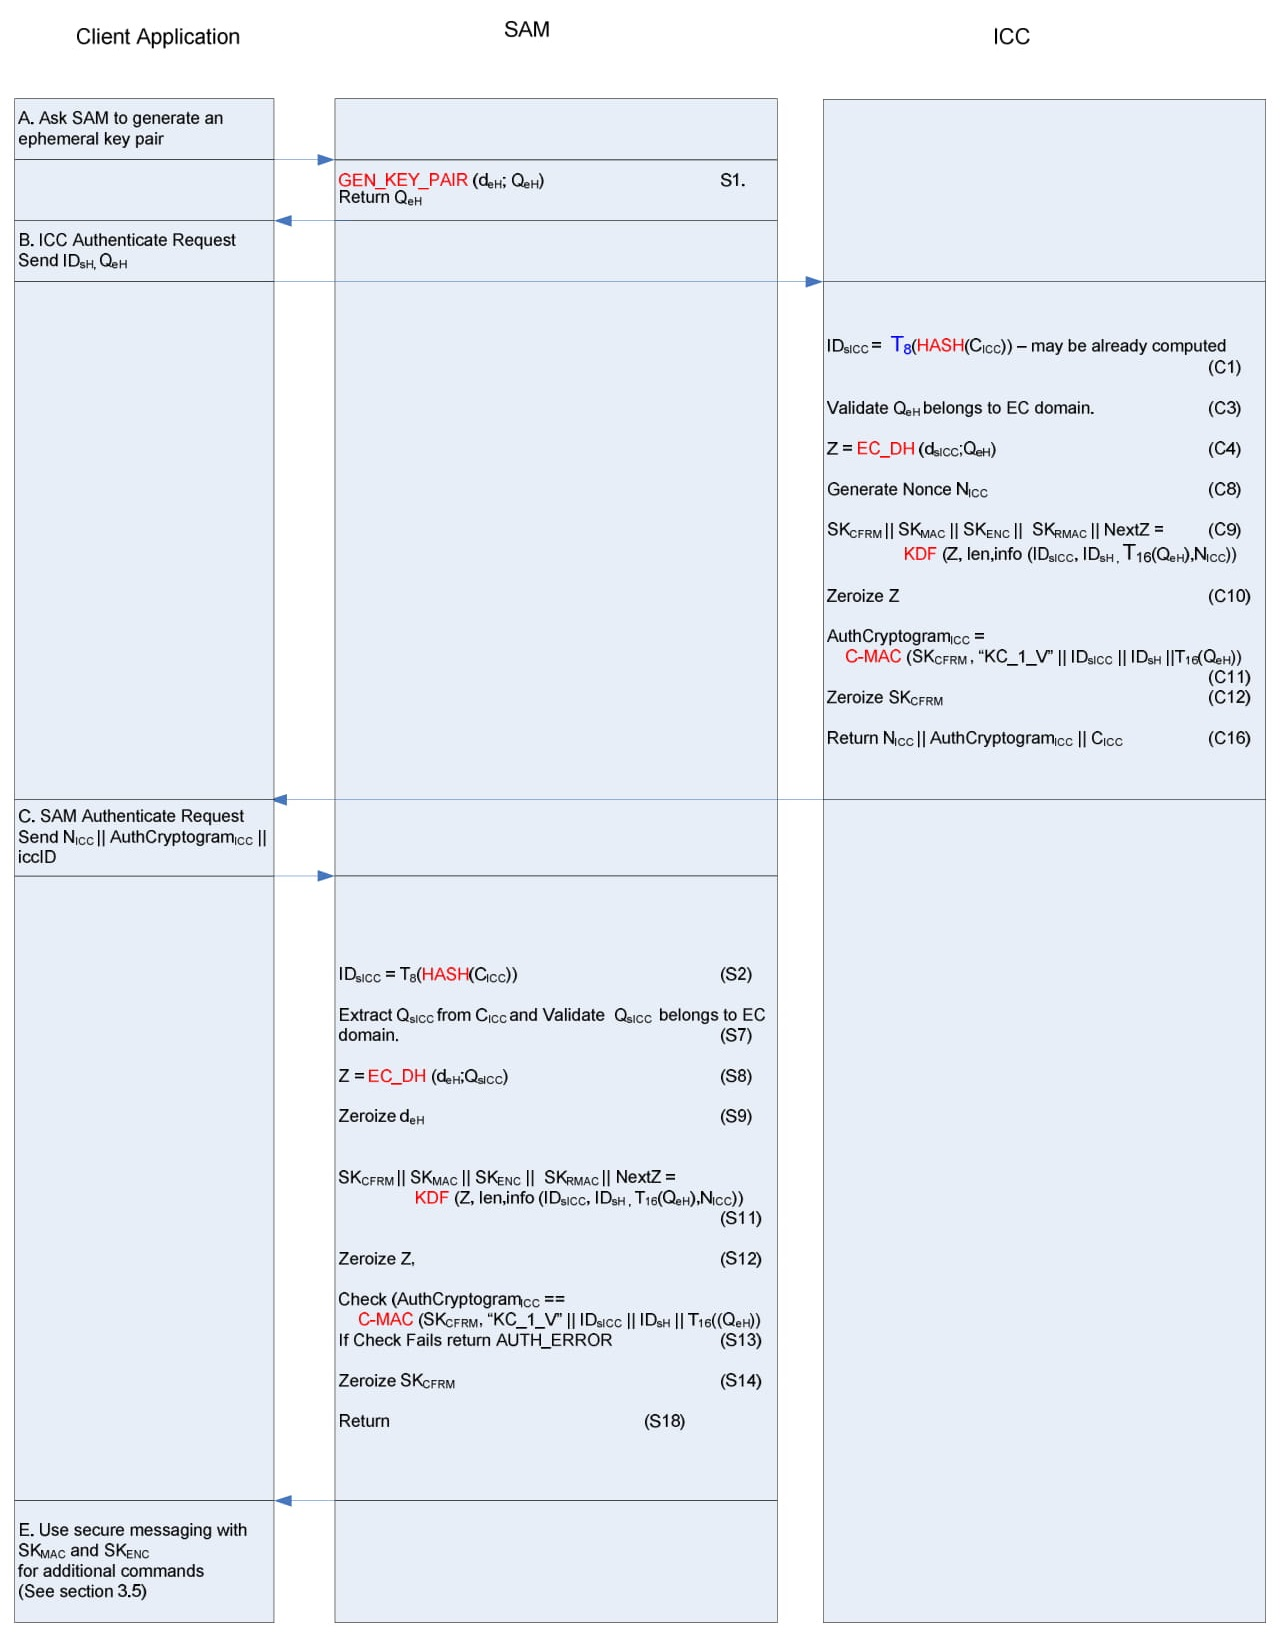
\includegraphics[scale=0.35]{appendix/opacity-zkm}
%	\caption{Base Opacity ZKM protocol timeline}
%	From the free Opacity specification \cite{opacityfree}
%\end{figure}

%\pagebreak
%\subsection{Appendix B - Opacity with Zero Key Management (ZKM-%Optimised)}
%\begin{figure} [ht]
%	\centering
%	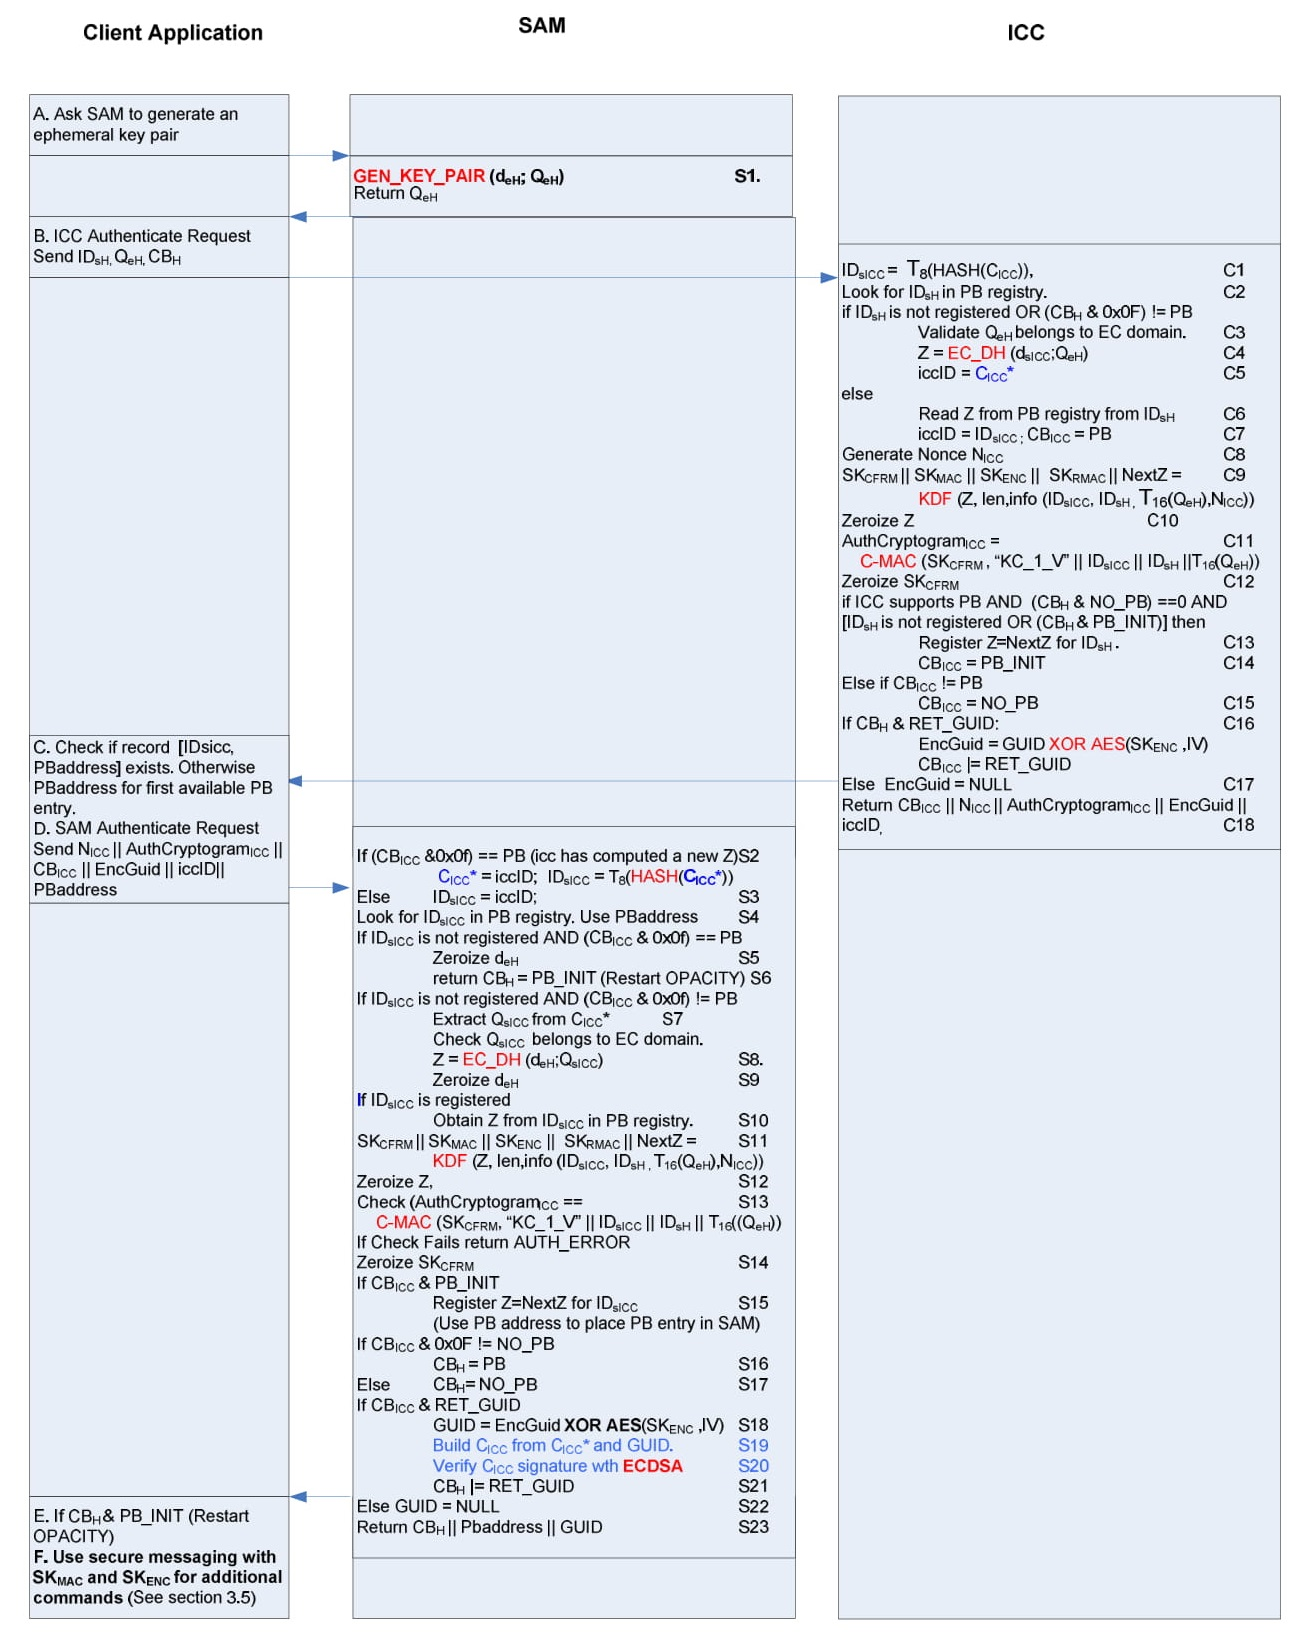
\includegraphics[scale=0.35]{appendix/opacity-zkm-opt}
%	\caption{Optimised Opacity ZKM protocol timeline}
%	From the free Opacity specification \cite{opacityfree}
%\end{figure}



\section{CVC format}
\label{cvc}
%TODO Reference where these are from.
\begin{figure} [ht]
	\center
	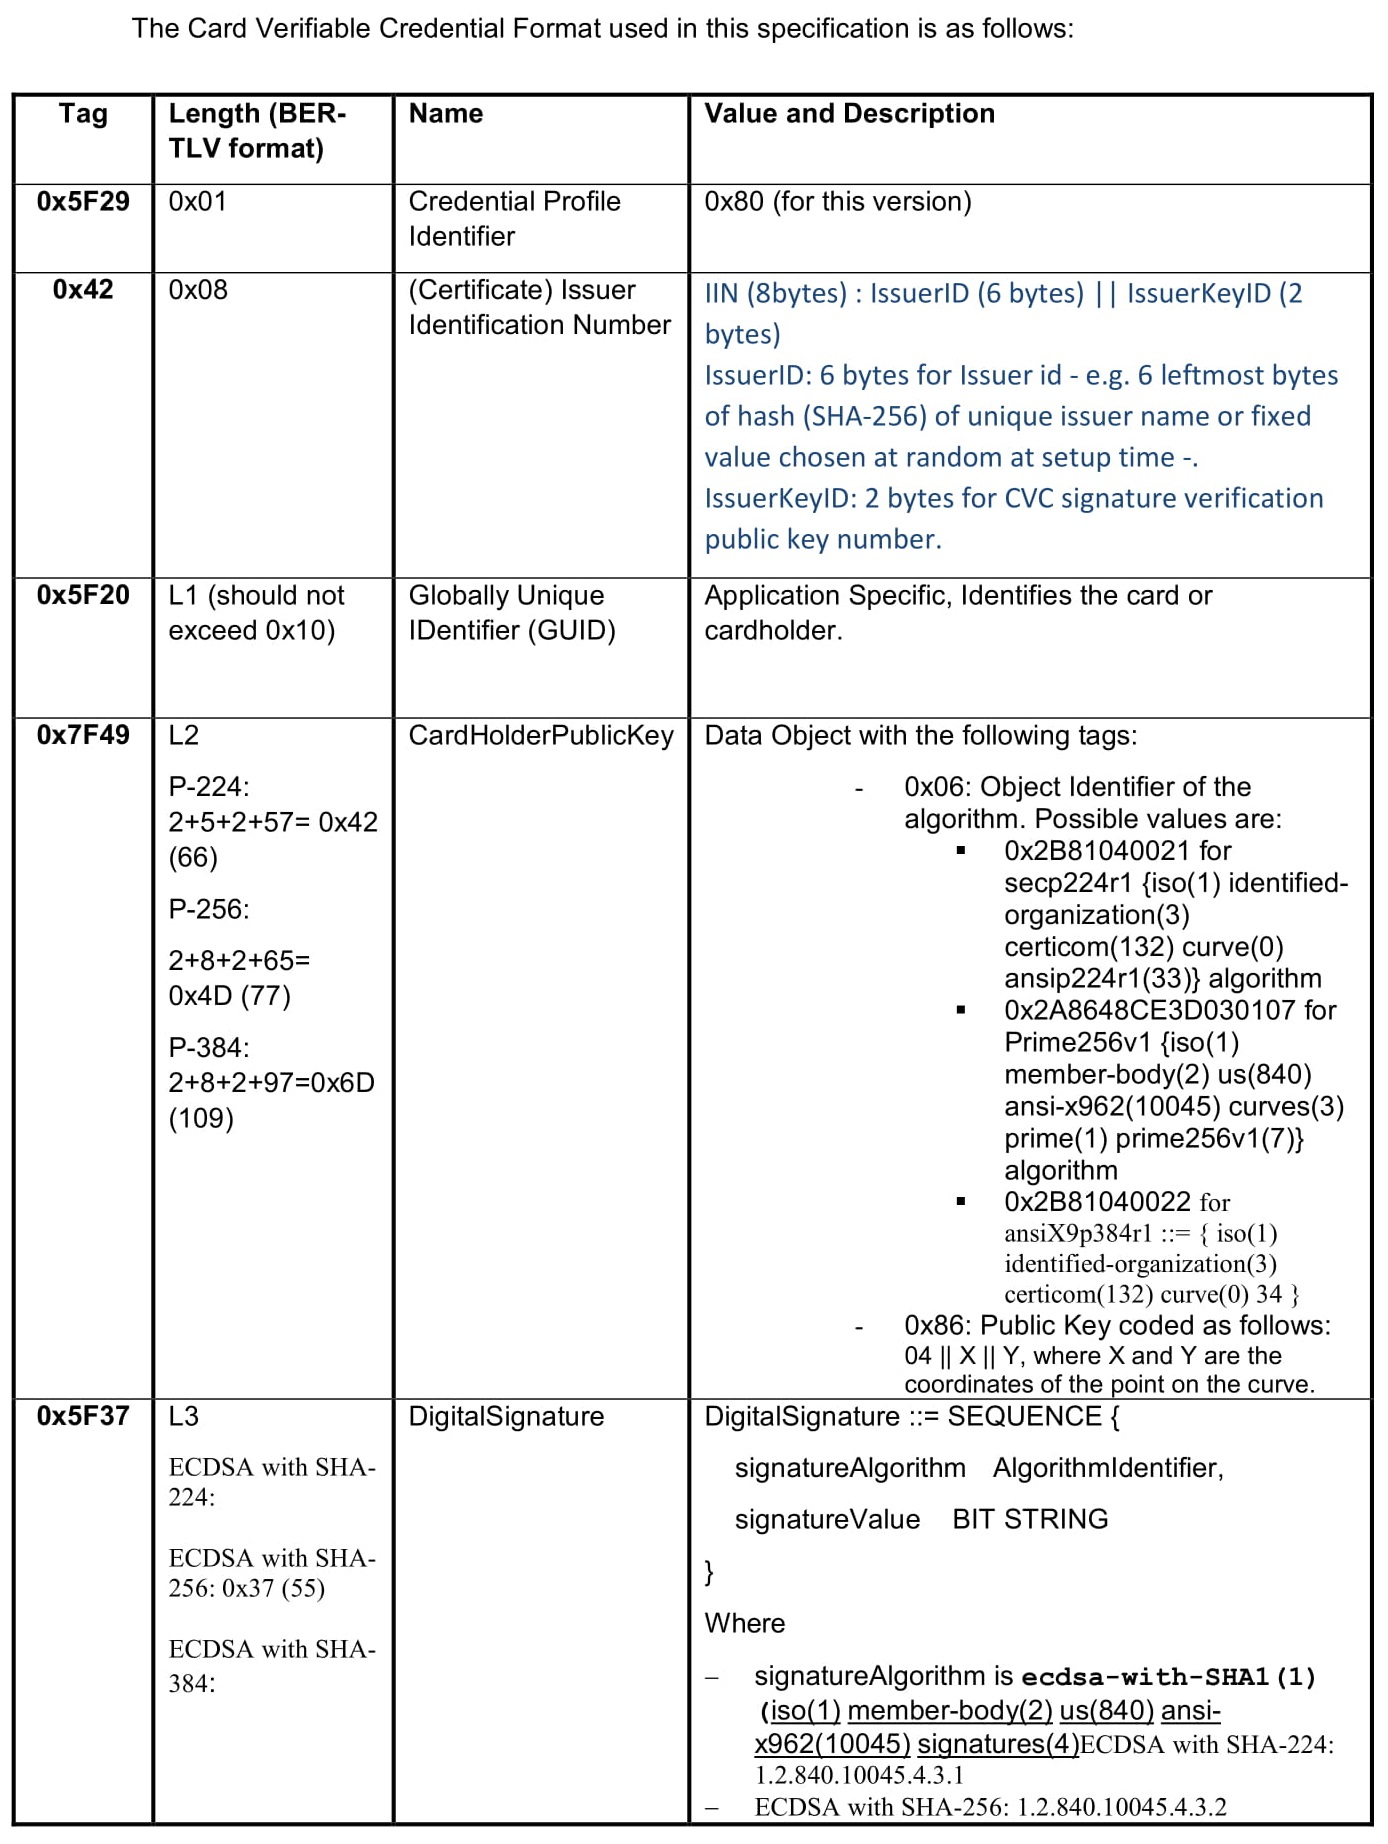
\includegraphics[scale=0.4]{appendix/cvc-1}
\end{figure}

\begin{figure} [h]
	\center
	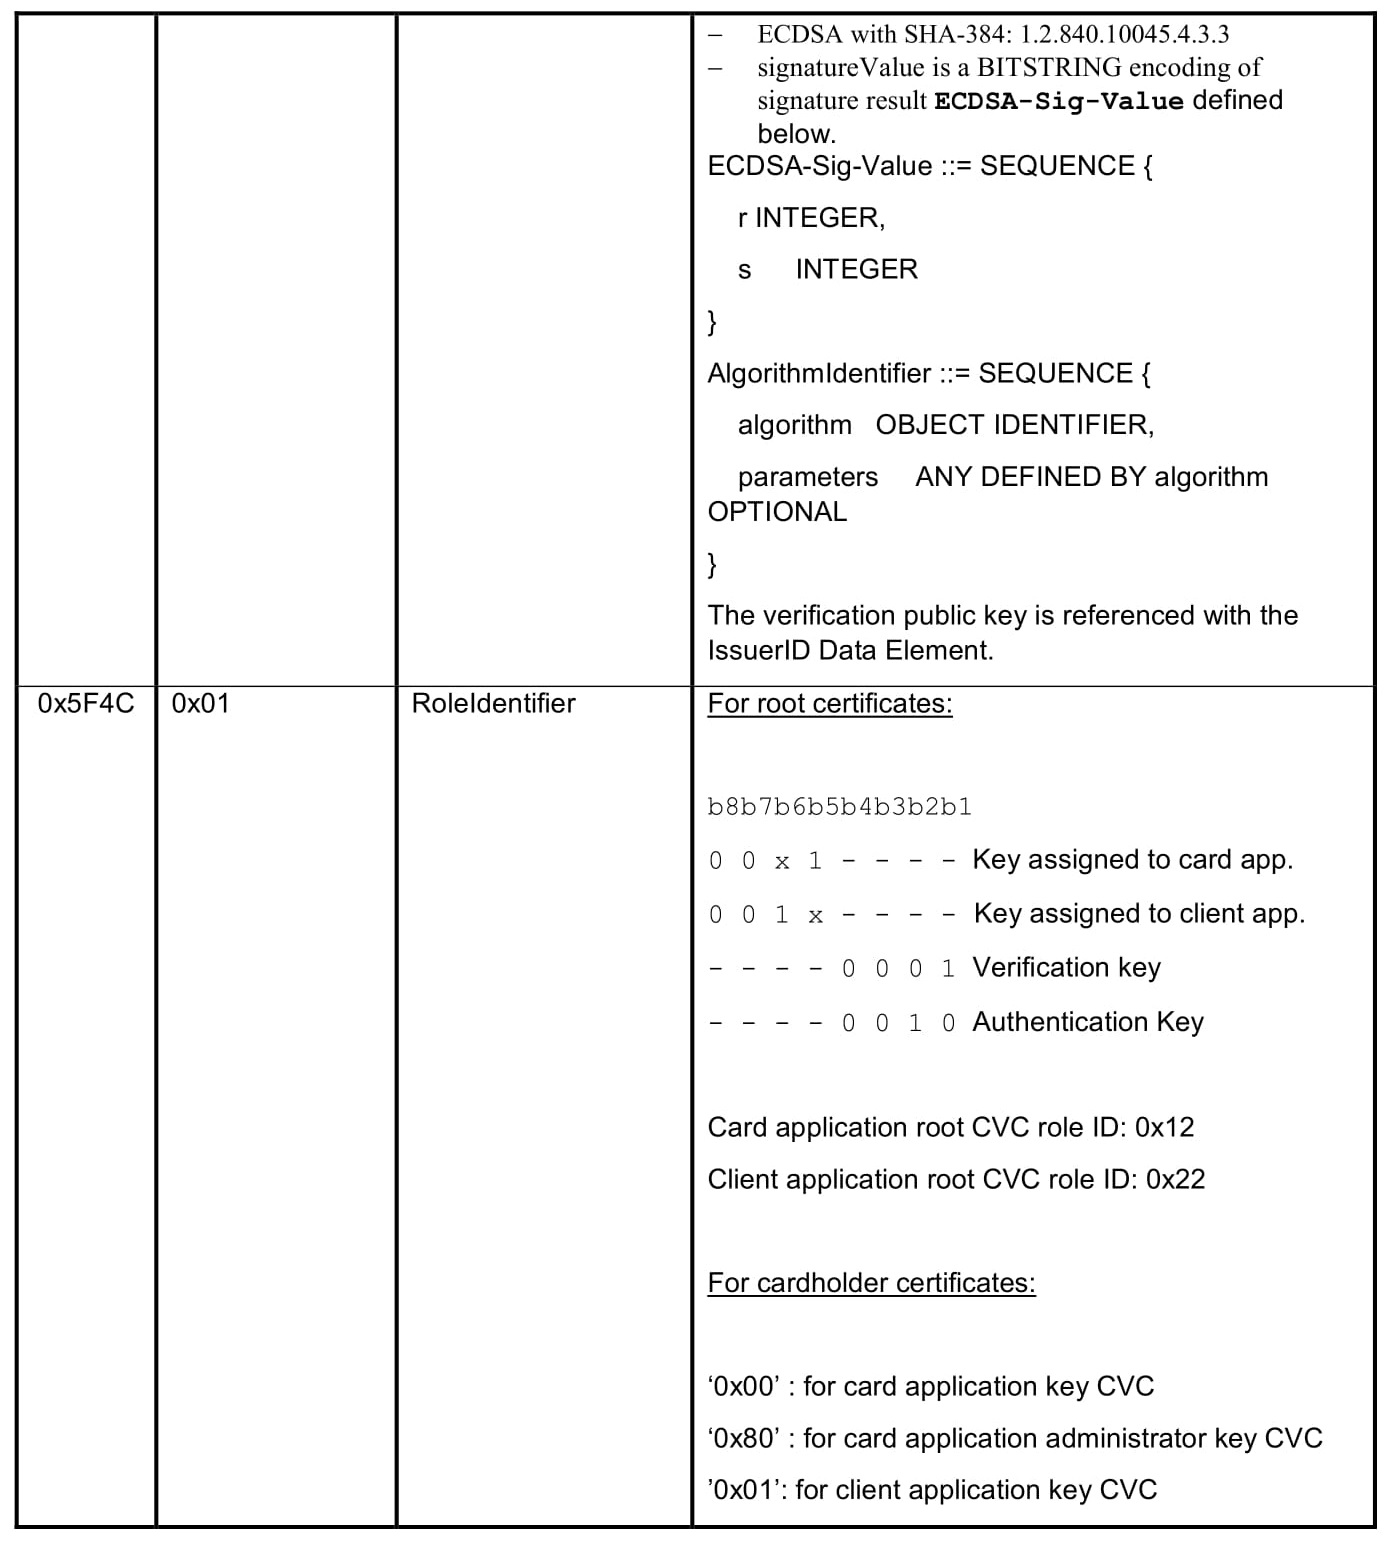
\includegraphics[scale=0.4]{appendix/cvc-2}
	
\end{figure}
\pagebreak
This is the Card Verifiable Credential (CVC) certificate format used in Opacity, taken from the free Opacity standard \cite{opacityfree}, section 8.0, annex B.

% TODO: Could include C-MAC steps from NIST 800-38B.

\pagebreak

\section{MIFARE Classic problems}
\label{sec:mifare_problems}

In December 2007, Henryk Pl\"otz and karsten Nohl gave a presentation describing the reverse-engineering of a hardware implementation of the MIFARE classic chip, and weaknesses they discovered. They published a full paper in August 2008. (TODO: links)

The pseudo-random number generator used for key generation among other things, is an NXP trade secret which was uncovered and shown to be fundamentally weak. It uses a 16b random number, blown up to 32b, to generate the initial state of a 48b Linear Feedback Shift Register. The initial random value depends on chip power-up time, so could be controlled. 

There is no nonlinear component in the LFSR feedback loop, so it can easily be reversed to find previously generated random numbers, to the system does not have forward-secrecy.

\begin{figure} [ht]
	\centering
	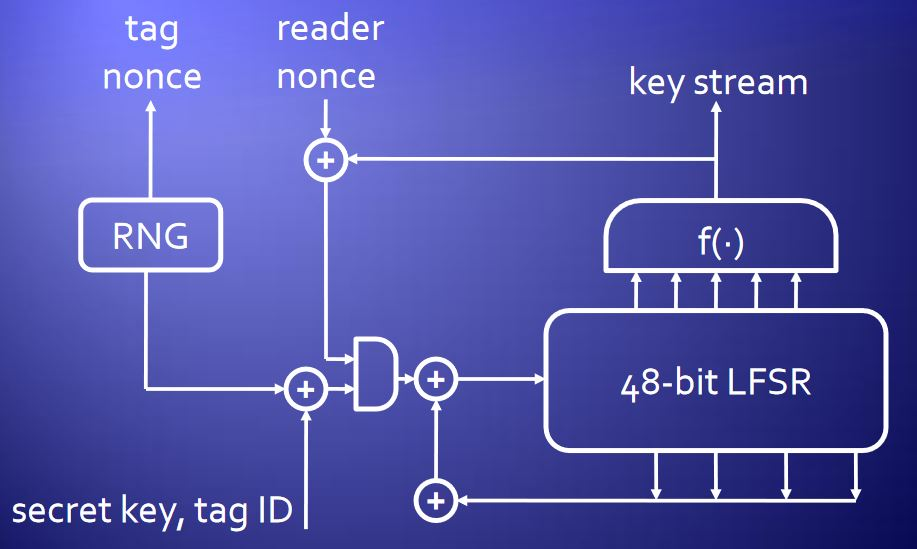
\includegraphics[scale=0.5]{introduction/mifare_classic.jpg}
	\caption{MIFARE Classic CRYPTO1 key generation algorithm}
	From Presentation \cite{TODO}
\end{figure}

The actual security of the keys is far less than the implied 48b. It ultimately depends on a 16b random number, which can be brute forced easily, but even better sub-exponential attacks may exist because each key stream bit is derived from a predetermined subset of values from the LFSR which suggests non-optimal avalanche properties. %Could explain further...

As this all suggests, the security of the card was dependent on obfuscation of the implementation details, which are now known, so the card is not insecure. By controlling randomness, an attacker can even generate duplicate cards with the same initial cipher state.

While Mifare classic may still be viable for protecting low-value things such as small payments, it isn't sufficient to protect higher-value targets e.g. credit cards or access control.

\subsection{Attacks}
Card memory is divided into sectors, each protected by two cryptographic keys. The reader must supply the keys in order to access the card's memory. In a typical Mifare system, all cards protected by the same keys. Recovery of a key makes the system vulnerable. As previously mentioned, the key generation process is weak

in a research group in Radbound University Nijmegen published four papers about their attacks on MIFARE classic. 

Among them, ``A practical attack on the MIFARE Classic" in which they extend the work of Nohl and Pl\"otz, exploiting the weakness in the pseudo-random generator to recover the CRYPTO1 keystream. They noted that nonces used to start the CRYPTO1 algorithm reappear four times per hour at 600,000 nonces per hour (though they can reappear in 0.618s if timing is exact) and used this to read the entire first sector, and show that they could read any sector provided that they know the content of one memory block in that sector.

Another of the papers is ``Wirelessly pickpocketing a MIFARE classic card" in which they outlined four attacks that only require a wireless reader, which are briefly summarised below:
\begin{enumerate}
	\item Mifare parity bits computed over plaintext, not cipher text, so they leak information. Only about 1500 authentication attempts necessary, then 48b offline brute-force attack to break the cipher.
	
	\item Also exploits parity bit weakness. Adaptive Chosen Ciphertext Attack with about 28500 adaptively chosen challenges to the card. Guarantees only 436 possibilities for odd-numbered bits of the internal cipher state. This reduces the offline search space to 33b.
	
	\item Attacker keeps challenge to the card constant, varying the challenge from the card to the reader until a special internal cipher state is reached. Special states are precomputed and placed in a 384GB table. Requires around 4096 authentication attempts, with a few extra for more efficient table lookup.
	
	\item Assume attacker has already recovered one sector key. Authenticate for that sector and then a new sector. Challenge nonce for new sector is encrypted with new sector key. Because of the 16b random number generator and that parity bits leak information, the attacker can easily calculate the plaintext nonce and hence 32b of the keystream. Use this to generate around $2^{16}$ candidate keys. Requires three authentication attempts and under a second offline search.
\end{enumerate}

Numerous other attacks have been used that are variations on the above. In April 2009, a better Conditional Multiple Differential card-only attack was found, first announced by Nicolas T. Courtois at Eurocrypt 2009.

\subsection{Problems with successors}
Some successor systems have also been shown to have security vulnerabilities.

In 2011, NXP replaced Mifare classic with the backwards compatible Mifare Classic EV1, which was resistant to the card-only attacks known at the time. However, a new card-only attack for the EV1 was found in 2015.

Mifare DESFire cards were shown to be insecure in 2010 when it was shown they could be cloned for about \$25 in easily available hardware. Other problems were also discovered.

Mifare Ultralight is also vulnerable to some attacks.

However, some newer AES-based systems such as the Mifare DESFire EV1 and Mifare Plus have not yet been broken.


\section{C-MAC explanation}
\label{cmac_expl}
A MAC, or Message Authentication Code, is a code that proves that a message was sent by the claimed sender, and was not modified in any way. It uses symmetric cryptography, so a MAC generated for a particular message by one party using a shared secret key can only be verified by another party also sharing this key, typically by also calculating the MAC of the message with that key and verifying it matches the received MAC.

\begin{figure} [ht]
	\centering
	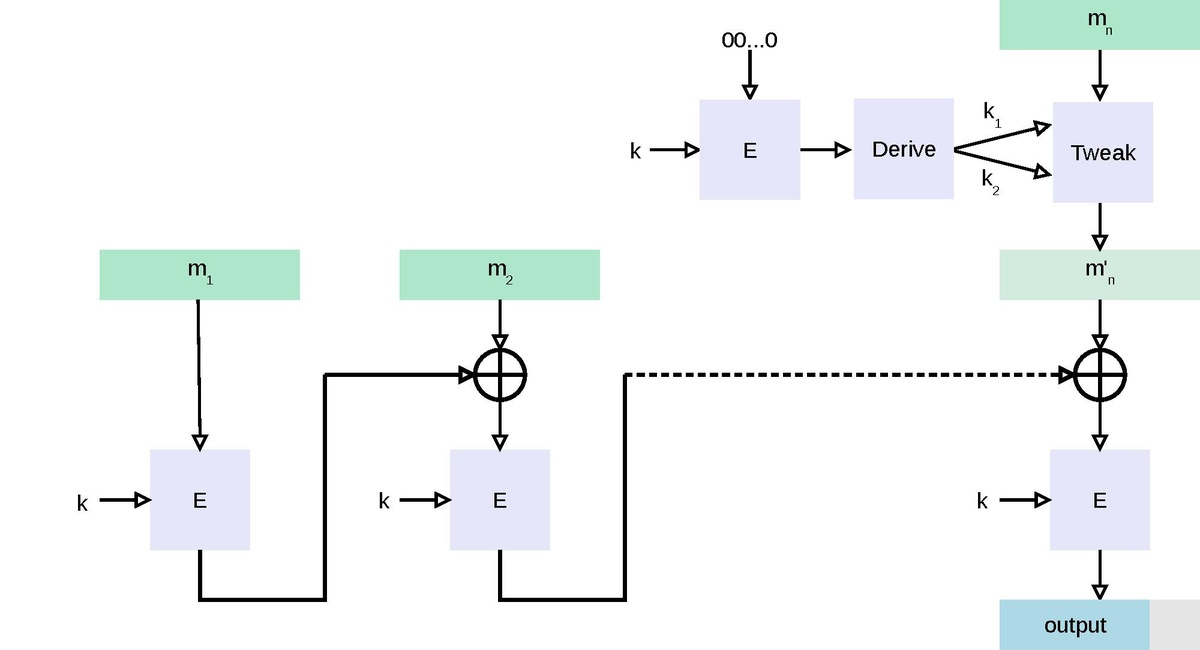
\includegraphics[scale=0.5]{implementation/CMAC}
	\caption{Diagram of C-MAC operation}
	From Wikipedia \cite{TODO}
\end{figure}

The best way to describe the C-MAC algorithm \cite{cmac} is to describe it as an extension of the CBC-MAC algorithm, which uses the CBC (Cipher Block Chaining) block cipher mode of operation. The link between the two can be easily seen by comparing the CMAC diagram with the following diagram outlining CBC-MAC:

\begin{figure} [ht]
	\centering
	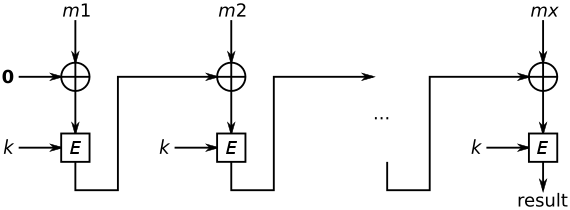
\includegraphics[scale=0.5]{implementation/CBC-MAC}
	\caption{Diagram of CBC-MAC operation}
	From Wikipedia \cite{TODO}
\end{figure}

Of course, $\mathbf{0} \oplus m1=m1$ so the initial step is identical to C-MAC. The difference is in the treatment of the final block of the message. In the CBC-MAC case, the final block is treated the same way all all the others, with the final cipherblock being used as the MAC.

%TODO wiki reference, this part is mostly copied from CBC-MAC Wikipedia page\\
This is secure for messages of an agreed fixed length, but not for variable-length messages. If two correct message-MAC pairs $(m,t)$ and $(m',t')$ are known, an attacker can generate a third message $m''$ with the MAC $t'$ as follows: 
$$m''=m||[[m'_1\oplus t] || m'_2 || \cdots \\ || m'_n]$$
This is because upon computation of $\text{MAC}(t)$, the MAC $t$ produced after $m$ has been processed will be XORed with $[m'_1 \oplus t]$, giving $m'_1$, and the rest of $m_1$ will be processed identically to if $m_1$ were processed by itself. C-MAC fixes this problem by XORing the final block $m_n$ with one of two subkeys derived from the primary key $k$ before executing CBC-MAC, which can't be replicated by the attacker who can't account for this step.


\pagebreak
\section{Partial Java Card C-MAC code}
\begin{verbatim}
// To initialise, save the key, and initialise the subkeys.
public void init(Key key, byte mode, byte[] init_info, short off, short len) {
    // If mode is verify, fail. Could be implemented but no need.

    // initialise CBC-MAC helper
    aesKey = (AESKey) key;
    Util.arrayFillNonAtomic(k, (short)0, (short)16, (byte)0x00);

    // Compute and store keys k1 and k2.
    aesKey.getKey(k, (short)0);
    Util.arrayFillNonAtomic(k1, (short)0, (short)16, (byte)0x00);

    aesCipher.init(aesKey, Cipher.MODE_ENCRYPT);

    // Generate subkeys
    aesCipher.doFinal(k1, (short)0, (short)16, k1, (short)0);
    subkeys(k1);
    Util.arrayCopy(k1, (short)0, k2, (short)0, (short)16);
    subkeys(k2);

    Util.arrayFillNonAtomic(prev_block, (short)0, (short)16, (byte)0x00);
    seen_data = false;

    // Initialise the block cipher with the key.
    aesCipher.init(aesKey, Cipher.MODE_ENCRYPT);
}

public short sign(byte[] input, short inOffset, short len, byte[] sigBuff, 
                  short sigOffset) {

    lastBlock = JCSystem.makeTransientByteArray((short)16, 
                                                JCSystem.CLEAR_ON_DESELECT);
    // Number of complete blocks (minus the last one if the last is complete)
    short leadingBlocks = (short)(len/16);  // Number of blocks before last.
    short lastBlockLen = (short)(len % 16);

    boolean no_data = !seen_data && len == 0;
    // Deal with special case of no input data. Pad block with 1 followed by
    // 0s and treat as single, complete block.

    if (lastBlockLen == 0 && !no_data) {
        // Overall input is a multiple of the block length.
        // Last block will be a full block.
        leadingBlocks--;
        lastBlockLen = 16;
    }
    short leadingBlocksLen = (short)(16 * leadingBlocks);

    // Step 4
    if (len != 0) {
        // Get last (possibly incomplete) block from sign() input
        Util.arrayCopy(input, (short)(inOffset + leadingBlocksLen), lastBlock,
                       (short)0, lastBlockLen);
    } else if (!no_data) {
        // Final input is last cached block provided to update()
        Util.arrayCopy(prev_block, (short)0, lastBlock, (short)0, (short)16);
    }
        
    // If no data was provided, lastBlock is a 0 block.
    if (lastBlockLen == 16) {
        // Last block takes up entire block, XOR it with k1
        for (short i = 0; i < 16; i++) {
            lastBlock[i] = (byte)(lastBlock[i] ^ k1[i]);
        }
    } else {
        // Pad last block with 1 followed by 0s and XOR with k2

        // Set the byte following the last data byte to 10000000
        lastBlock[lastBlockLen] = (byte)0x80;
        // Set all later bytes to 0.
        for (short i = (short)(lastBlockLen + 1); i < 16; i++) {
            lastBlock[i] = 0x00;
        }

        // Now XOR entire block with k2.
        for (short i = 0; i < 16; i++) {
            lastBlock[i] = (byte)(lastBlock[i] ^ k2[i]);
        }
    }

    // If the last block comes from the sign() input, update with prev_block
    if (len != 0) {
        if (leadingBlocksLen != 0) {
            // Pass the leading blocks to the cipher if there are any.
            update(input, inOffset, leadingBlocksLen);

            // Cipher the cached block (second last block).
            aesCipher.update(prev_block, (short)0, (short)16, temp, (short)0);
        }
    }

    aesCipher.doFinal(lastBlock, (short)0, (short)16, sigBuff, sigOffset);

    return 16;
}
\end{verbatim}

\pagebreak
\section{Timing tables}
In analysing the timing of the card-side protocol implementation, I placed code at different points in the protocol that ended execution based on the APDU parameters, and modified the host-side application to make many authentication attempts with different parameter values, recording the time taken for the smartcard to return. 

The break points, referring to various points within the protocol (Appendix TODO), are as follows:
\begin{enumerate}
	\item Return immediately, gives connection overhead.
	\item Return after initial array allocation.
	\item Return after shared secret is acquired, either by EC-DH or PB registry lookup.
	\item Return after nonce is generated.
	\item Return after the session keys are generated.
	\item Return after various array operations.
	\item Return after the CMAC authentication code is calculated.
	\item Return after the entire protocol has finished execution.
\end{enumerate}

Note that running with \verb|PB_INIT| takes fractionally longer than NO\_PB because of the time to create a new PB record, but doesn't differ enough to warrant more tables.

\subsection{Initial implementation}
\label{subsec:init_timings}

\begin{table} [ht]
\begin{center}
\begin{tabular}{|c|c|c|c|c|c|c|c|c|}
	\hline
	Time(s) & 1     & 2    & 3    & 4    & 5    & 6    & 7    & 8\\
	\hline
	1       & 0.06  & 0.27 & 0.77 & 0.85 & 1.74 & 1.89 & 3.12 & 3.21\\
	2       & 0.07  & 0.27 & 0.77 & 0.85 & 1.74 & 1.89 & 3.12 & 3.22\\
	3       & 0.07  & 0.27 & 0.77 & 0.85 & 1.74 & 1.89 & 3.12 & 3.22\\
	average & 0.07  & 0.27 & 0.77 & 0.85 & 1.74 & 1.89 & 3.12 & 3.22\\
	\hline
\end{tabular}
\caption{Initial implementation, base protocol}
\end{center}
\end{table}

\begin{table} [ht]
\begin{center}
\begin{tabular}{|c|c|c|c|c|c|c|c|c|}
	\hline
	Time(s) & 1     & 2    & 3    & 4    & 5    & 6    & 7    & 8\\
	\hline
	1       & 0.07  & 0.28 & 0.27 & 0.36 & 1.27 & 1.43 & 2.63 & 2.71\\
	2       & 0.07  & 0.28 & 0.27 & 0.36 & 1.27 & 1.43 & 2.63 & 2.71\\
	3       & 0.07  & 0.28 & 0.27 & 0.36 & 1.27 & 1.43 & 2.63 & 2.72\\
	average & 0.07  & 0.28 & 0.27 & 0.36 & 1.27 & 1.43 & 2.63 & 2.71\\
	\hline
\end{tabular}
\caption{Initial implementation, with Persistent Binding enabled}
\end{center}
\end{table}

\pagebreak
\subsection{After optimisations}
%TODO: Should I include intermediate measurements after 1st round of optimisations?
\begin{table} [h]
\begin{center}
\begin{tabular}{|c|c|c|c|c|c|c|c|c|}
	\hline
	Time(s) & 1      & 2    & 3     & 4    & 5    & 6    & 7    & 8\\
	\hline
	1       & 0.065  & 0.065 & 0.23 & 0.24 & 0.24 & 0.24 & 0.68 & 0.75\\
	2       & 0.065  & 0.066 & 0.24 & 0.24 & 0.24 & 0.24 & 0.68 & 0.74\\
	3       & 0.064  & 0.065 & 0.24 & 0.24 & 0.24 & 0.24 & 0.67 & 0.75\\
	average & 0.065  & 0.065 & 0.24 & 0.24 & 0.24 & 0.24 & 0.68 & 0.75\\
	\hline
	
\end{tabular}
\caption{After code optimisations, base protocol}
\end{center}
\end{table}

\begin{table}
\begin{center}
\begin{tabular}{|c|c|c|c|c|c|c|c|c|}
	\hline
	Time(s) & 1      & 2     & 3     & 4     & 5    & 6    & 7    & 8\\
	\hline
	1       & 0.065  & 0.065 & 0.066 & 0.067 & 0.073 & 0.073 & 0.52 & 0.58\\
	2       & 0.065  & 0.066 & 0.067 & 0.067 & 0.073 & 0.073 & 0.51 & 0.57\\
	3       & 0.065  & 0.066 & 0.066 & 0.067 & 0.073 & 0.073 & 0.51 & 0.58\\
	average & 0.065  & 0.066 & 0.066 & 0.067 & 0.073 & 0.073 & 0.51 & 0.58\\
	\hline
\end{tabular}
\caption{After code optimisations, with persistent Binding enabled}
\end{center}
\end{table}



\pagebreak

%TODO could optionally do index
%Index


\pagebreak
%Bibliography
\begin{thebibliography}{9}
	\bibitem{pcsc}
	PC/SC Workgroup,\\
	\texttt{https://www.pcscworkgroup.com/}
	
	\bibitem{opacityfree}
	Outdated but free Opacity standard,\\
	\texttt{https://www.securetechalliance.org/resources/pdf/OPACITY\char`_Protocol\char`_3.7.pdf}
	
	\bibitem{opacity}Official Opacity specification, \\
	\textit{ANSI INCITS 504-1-2013 Information technology – Generic Identity Command Set – Part 1: Card Application Command Set}
	
	\bibitem{ec_diagram}
	Elliptic Curve diagram used in this dissertation,\\
	\texttt{https://stackoverflow.com/questions/19800518/ \\
	python-matplotlib-for-elliptic-curve-with-sympy-solve}
	
	\bibitem{p256}
	NIST recommended Elliptic Curve parameters for the P-256 curve,\\
	\textit{FIPS Pub 186-4, Digital Signature Standard (DSS), appendix D.1.2.3 Curve P-256}\\
	\texttt{https://nvlpubs.nist.gov/nistpubs/FIPS/NIST.FIPS.186-4.pdf}
	
	\bibitem{cmac}
	Definition of the C-MAC mode for authentication,\\
	\textit{NIST 800-38B, Recommendation for Block Cipher Modes of Operation: The CMAC Mode for Authentication}\\
	\texttt{https://nvlpubs.nist.gov/nistpubs/SpecialPublications/NIST.SP.800-38B.pdf}
	
	\bibitem{ocf}
	OpenCard Framework,\\
	\texttt{https://www.openscdp.org/ocf/}
	
	\bibitem{generic_costs}
	CardWerk overview of typical characteristics of smartcard systems, including costs\\
	\verb|http://cardwerk.com/smart-card-technology/|
	
	\bibitem{card}
	ACOSJ 40K dual interface Java Card, (Java Card version 3.0.4)\\
	\verb|https://www.smartcardfocus.com/shop/ilp/id~790/acosj-dual-interface-java-card/|
	\verb|p/index.shtml|
	
	
	\bibitem{reader}
	Identive SCL3711 USB card reader, used in this project\\
	\verb|https://www.smartcardfocus.com/shop/ilp/id~387/scl3711/p/index.shtml|

	\bibitem{gpshell}
	GPShell, a scripting tool for managing smartcard applets according to the GlobalPlatform specifications\\
	\verb|https://sourceforge.net/p/globalplatform/wiki/GPShell/|
	
	\bibitem{globalplatform}
	GlobalPlatform, a set of specifications for how applets are managed on a smartcard (amongst other related things)\\
	\verb|https://www.globalplatform.org/specifications.asp|
	
	\bibitem{pyscard}
	Pyscard, a PC/SC API for Python,\\
	\verb|https://pyscard.sourceforge.io/|
	
	\bibitem{birthday}
	Birthday problem (a.k.a. birthday paradox),\\
	\verb|https://en.wikipedia.org/wiki/Birthday_problem|
	
	\bibitem{facebook_onion}
	Example of brute-force search for a public key with desirable properties,\\
	\verb|https://en.wikipedia.org/wiki/Facebookcorewwwi.onion|
	
	\bibitem{jcdk_guide}
	Java Card 2.2.2 User's Guide,\\
	\textit{Sun microsystems Development Kit User's Guide for the binary release with cryptography extensions, Java Card platform, version 2.2.2}\\
	\verb|https://usermanual.wiki/Pdf/cJDKUsersGuidebindo.534662277.pdf|
\end{thebibliography}

\end{document}



